\documentclass[oneside,final,14pt,a4paper]{extreport}

\usepackage{tgtermes} % Times New Roman alike font

\usepackage{vmargin}
\setpapersize{A4}
\setmarginsrb{2.5cm}{2.0cm}{2.0cm}{2.0cm}{0pt}{10mm}{0pt}{13mm}
\usepackage{setspace}
\setstretch{1.5}
\usepackage{indentfirst}
\parindent=1.25cm

%%%%% ADDED TO SUPPORT TT BOLD FACES %%%%
\DeclareFontShape{OT1}{cmtt}{bx}{n}{<5><6><7><8><9><10><10.95><12><14.4><17.28><20.74><24.88>cmttb10}{}
\renewcommand{\ttdefault}{pcr}
%%%%% END %%%%%%%%%%%%%%%%%%%%%%%%%%%%%%%

\usepackage{atbegshi,picture}
\usepackage{cmap}
\usepackage[T1]{fontenc}
\usepackage[utf8]{inputenc}

\usepackage[english]{babel}
\usepackage[backend=biber,style=ieee,autocite=inline]{biblatex}
\addbibresource{ref.bib}
\DefineBibliographyStrings{english}{%
  bibliography = {References},}
\usepackage{pdfpages}
\newenvironment{bottompar}{\par\vspace*{\fill}}{\clearpage}
\usepackage{amsmath,amsfonts}
\usepackage{url}
\usepackage{xurl}
\usepackage{amsthm}
\newtheorem{theorem}{Theorem}
\newtheorem{corollary}{Corollary}
\newtheorem{lemma}{Lemma}
\newtheorem{proposition}{Proposition}
\theoremstyle{definition}
\newtheorem{definition}{Definition}
\theoremstyle{remark}
\newtheorem*{remark}{Remark}
\theoremstyle{remark}
\newtheorem*{example}{Example}


\usepackage{float}
\usepackage{graphicx}
\graphicspath{{figs/}} %path to images
\usepackage{array}
\usepackage{multirow}
\usepackage[font=singlespacing, labelfont=bf]{caption}
\usepackage{subcaption}
\usepackage{paralist}
\usepackage{listings}
\usepackage{zed-csp}
\usepackage{fancyhdr}
\usepackage{csquotes}
\usepackage{color}

% \usepackage{anyfontsize}
% \usepackage{mathptmx}
% \usepackage{t1enc}

\usepackage{chngcntr}
\usepackage{upgreek}
\usepackage{bm}
\usepackage{booktabs}
\usepackage{longtable}
\usepackage{pgfplots}
\pgfplotsset{compat=1.18}
% MY PACKAGES%
\usepackage{tabularx}
\usepackage{pdflscape}
\usepackage{verbatim}
\lstset{
  basicstyle=\ttfamily\small,
  columns=fullflexible,
  keepspaces=true,
  frame=single,
  breaklines=true
}

% END %
%Hints
\newcommand\pic[1]{(Fig. \ref{#1})} %Ref on figure
\newcommand\tab[1]{(Tab. \ref{#1})} %Ref on table

\setlength{\headheight}{32.0976pt}
\usepackage{enumitem}
\newlist{inlinelist}{enumerate*}{1}
\setlist*[inlinelist,1]{%
  label=(\arabic*),
}

% \setcounter{secnumdepth}{4}
\captionsetup[table]{labelfont={normalfont}, name={TABLE}, labelsep={newline}, justification=centering}
\setlength{\parindent}{1.25cm}
\DeclareCaptionLabelSeparator{figSep}{.\quad}
\captionsetup[figure]{labelfont={normalfont}, name={Fig.}, labelsep=period, justification=raggedright, singlelinecheck=false}
\counterwithin{figure}{chapter}

% \usepackage{titlesec}
% \titleformat{\section}[hang]{\fontsize{20}{24}\selectfont\filcenter}{\Roman{section}}{1em}{}
% \titleformat{\subsection}[hang]{\itshape}{\Alph{subsection}.}{1em}{}[]
% \titleformat{\subsubsection}[runin]{\itshape}{\arabic{subsubsection})}{1em}{}[$:$]
% \titlespacing{\subsubsection}{1em}{1em}{1em}
% \titleformat{\paragraph}[runin]{\itshape}{\alph{paragraph})}{1em}{}[$:$\quad]
% \titlespacing{\paragraph}{2em}{1em}{1em}

\usepackage{placeins} % for \FloatBarrier
\usepackage[hidelinks]{hyperref}
\setcounter{biburlnumpenalty}{9000}
\setcounter{biburlucpenalty}{9000}
\setcounter{biburllcpenalty}{9000}
\emergencystretch=2em

\pagestyle{fancyplain}

\fancypagestyle{plain}{%
  \fancyhf{}%
  \rhead{\bfseries\thepage}%
  \renewcommand{\headrulewidth}{0pt}%
  \renewcommand{\footrulewidth}{0pt}%
}

% remember section title
\renewcommand{\chaptermark}[1]%
	{\markboth{\chaptername~\thechapter~--~#1}{}}

% subsection number and title
\renewcommand{\sectionmark}[1]%
	{\markright{\thesection\ #1}}

\rhead[\fancyplain{}{\bf\leftmark}]%
      {\fancyplain{}{\bf\thepage}}
\lhead[\fancyplain{}{\bf\thepage}]%
      {\fancyplain{}{\bf\rightmark}}
\cfoot{} %bfseries


\newcommand{\dedication}[1]
   {\thispagestyle{empty}

   \begin{flushleft}\raggedleft #1\end{flushleft}
}

\begin{document}
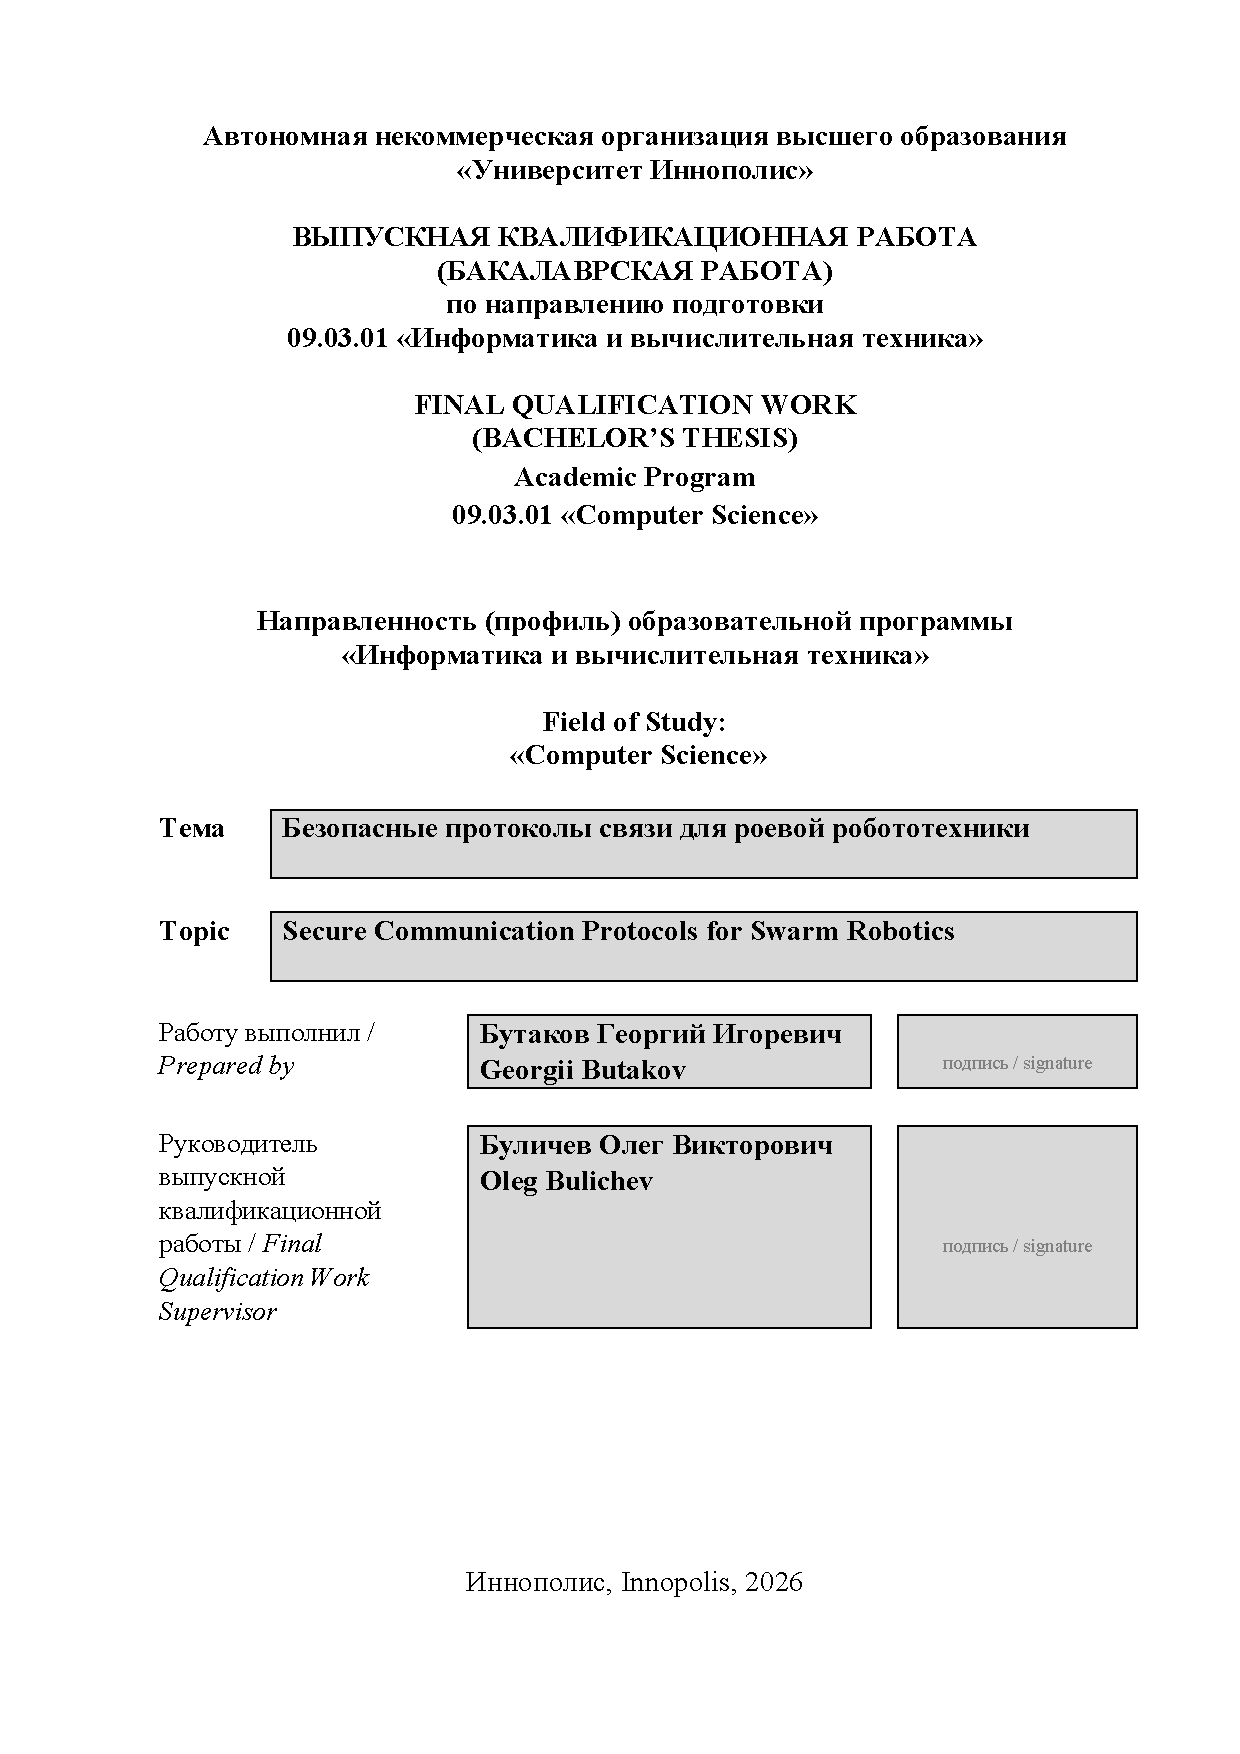
\includepdf[pages=-, offset=72 -72]{title.pdf}
\tableofcontents
\listoftables
\listoffigures
\newpage


%\begin{abstract}
This thesis develops and evaluates an adaptive lightweight secure-communication
framework for swarm-oriented systems. The proposed architecture maps runtime
state indicators to cryptographic profiles and uses X25519-based session
establishment, AEAD payload protection, and lightweight runtime authentication.
The executable evaluation focuses on a constrained pairwise prototype running in
containers, where static-heavy, static-balanced, static-lightweight, and
adaptive modes are compared under CPU, rekeying, and network-impairment
conditions.

The benchmark results show that lightweight mode provides the best measured
throughput and the lowest normalized model-based energy proxy under the tested
compute constraint, while adaptive mode correctly switches between profiles and
acts as a policy-driven compromise rather than a universally optimal mode. The
results are intentionally bounded: they validate data-plane behavior in a
host-based prototype, not a complete deployed multi-hop robotic swarm.
\end{abstract}



\chapter{Introduction}
\label{chap:intro}

Swarm robotics studies how many relatively simple agents can coordinate through local interaction without continuous centralized control~\cite{diasSwarmRoboticsPerspective2021,debieSwarmRoboticsSurvey2023}. In practice, that coordination depends on message exchange over dynamic wireless links, so communication reliability and communication security become intertwined design concerns rather than separate subsystems~\cite{varadharajanSwarmRelaysDistributed2020,chenSecuringEmergentBehaviour2021}.

The literature reviewed in this thesis suggests a recurring trade-off. Lightweight cryptographic mechanisms are attractive for constrained UAV and IoT-style platforms because they reduce key size, messaging overhead, and runtime cost~\cite{adeniyiSystematicReviewECC2024,hanLightweightSecureCommunication2025,manikandanASMTPAnonymousSecureMessaging2024}. At the same time, stronger decentralized trust mechanisms, such as blockchain-assisted coordination or attestation frameworks, can improve system assurance but usually add latency, bandwidth cost, or implementation complexity~\cite{sunResearchDataSecurityEmergency2022,pachecoSecuringFederatedLearning2024,kohliSwarmNetFirmwareAttestation2024}. Within this representative corpus, adaptive control of cryptographic settings is discussed less often than the underlying primitives themselves.

This thesis addresses that narrower gap by developing and evaluating an adaptive lightweight communication framework that dynamically balances security-oriented settings and performance-oriented settings in a swarm-inspired environment. The relevance of the topic follows from the growing use of distributed robotic and IoT-style systems in settings where communication must remain protected even when energy, bandwidth, and processing capacity are limited.

The purpose of the thesis is to design and evaluate a reproducible adaptive secure-communication framework for swarm-oriented systems. The main tasks are to review relevant swarm-security and lightweight-cryptography literature, define a formal model and threat model, specify adaptive cryptographic profiles, implement a pairwise benchmark prototype, and compare static-heavy, static-balanced, static-lightweight, and adaptive operation under constrained execution.

The object of study is secure communication in swarm-oriented distributed systems. The subject of study is adaptive selection of cryptographic profiles for the protected data plane. The scientific novelty of the work is the combination of a bounded formal model with an executable benchmark that exposes the security--performance trade-off instead of treating the adaptive framework only as a conceptual architecture.

The swarm network is modeled as a dynamic graph $G(V,E,t)$, and the adaptation function
\begin{equation}
F : S(t) \rightarrow P,
\label{eq:adaptation_function}
\end{equation}
maps swarm-state variables $S(t)$ to configurable cryptographic parameters $P$. At the conceptual level, $S(t)$ includes density, energy, packet loss, and threat estimates, while $P$ includes key length, cipher selection, authentication mode, and key-rotation frequency. At the executable level, the benchmark prototype instantiates a smaller pairwise subset of this idea: it switches between three runtime profiles using scripted threat and energy inputs and evaluates the resulting data-plane behavior under constrained CPU and memory budgets.

The contribution is therefore twofold. First, the thesis develops a formal and architectural model for adaptive secure communication in swarm-oriented systems. Second, it grounds that model in a reproducible pairwise benchmark prototype instead of relying only on analytical estimates. The implementation artifacts, scenario presets, tests, and final benchmark matrix are organized as a reproducible repository artifact accompanying the thesis. The resulting evidence is intentionally narrower than a field deployment: it supports claims about the behavior of a constrained host-based prototype, not about full multi-hop swarm operation on physical robots.

\chapter{Literature Review}
\label{chap:lr}

This chapter is a representative review of recent works most directly related to the thesis problem statement. It is not intended as a systematic review of the full swarm-security literature; instead, it synthesizes a focused corpus covering swarm communication, lightweight cryptography, decentralized trust, and adaptive security.

\section{Communication Architectures of Swarm Systems}
\label{sec:swarm_comm_arch}

Swarm robotics is grounded in self-organization, local interaction, and emergent collective behavior. Surveys by Dias et al.~\cite{diasSwarmRoboticsPerspective2021} and Debie et al.~\cite{debieSwarmRoboticsSurvey2023} show that scalability and fault tolerance are central advantages of swarm systems, but they also make reliable communication a critical dependency.

Varadharajan et al.~\cite{varadharajanSwarmRelaysDistributed2020} addressed connectivity in dynamic environments through the \textit{Swarm Relays} algorithm, which builds distributed self-healing communication chains across heterogeneous robots. Arseneault et al.~\cite{arseneaultRASSRiskAwareSwarm2022} proposed \textit{RASS}, a risk-aware storage framework that distributes replicas according to environmental hazard. Together, these studies show that decentralized coordination and survivability can be achieved without centralized infrastructure, but they leave confidentiality and authentication only partially addressed.

Swarm network topologies vary from mesh to cluster-based configurations in order to manage connectivity and scalability. Mesh topologies provide path redundancy and self-recovery under node failures; star structures centralize information flow, simplifying key management at the cost of a single point of failure; cluster-based organization balances local autonomy with hierarchical coordination, reducing communication overhead.

Topology selection influences attack resilience: mesh networks resist selective interception but require complex key management; star systems are vulnerable to compromise of the central node; cluster-based architectures localize damage but require secure inter-cluster communication channels.

Self-healing communication chains maintain continuous network coverage under dynamic changes. Robots autonomously reconfigure links by detecting disruptions and establishing alternative routes. Risk-aware storage and routing approaches further improve resilience by placing critical data away from high-risk regions of the swarm~\cite{arseneaultRASSRiskAwareSwarm2022}.

These approaches establish an important foundation for robust swarm networking, yet they do not by themselves provide a complete secure communication stack. Encryption, authentication, and adaptive key management are still required to protect the information exchanged over these resilient topologies, as summarized in Table~\ref{tab:comm_arch_comparison}.

\begin{table}[H]
\centering
\caption{Comparison of communication architectures of swarm systems}
\label{tab:comm_arch_comparison}
\scriptsize
\renewcommand{\arraystretch}{1.14}
\begin{tabularx}{\textwidth}{|p{2.2cm}|p{2.4cm}|p{2.0cm}|X|p{2.5cm}|}
\hline
\textbf{Architecture} & \textbf{Topology} & \textbf{Fault Tolerance} & \textbf{Security Integration} & \textbf{Application} \\
\hline
Swarm Relays & Hybrid mesh-chain & High & Connectivity oriented, no built-in encryption & Ground--air heterogeneous swarms \\
\hline
RASS & Cluster-based & Medium & Risk awareness without message confidentiality & Distributed data storage \\
\hline
Mesh topology & Fully connected & High & Requires complex key management & Large-scale UAV swarms \\
\hline
Star topology & Centralized & Low & Simplified, single point of failure & Small specialized groups \\
\hline
Cluster-based & Hierarchical & Medium & Inter-cluster protection required & Multi-level heterogeneous systems \\
\hline
\end{tabularx}
\end{table}

This comparison highlights a recurring design tension: the architectural choices that improve robustness often complicate secure message exchange. That tension motivates lightweight, decentralized cryptographic mechanisms that can operate within the same resource envelope as the swarm itself.

\section{Lightweight Cryptography}
\label{sec:lightweight_crypto}

Lightweight cryptography for constrained agents has been extensively studied. Han et al.~\cite{hanLightweightSecureCommunication2025} show that elliptic-curve methods remain attractive for UAV swarms because they reduce key size and communication overhead relative to conventional PKI while still supporting authenticated key establishment.

Symmetric authenticated encryption provides the practical data-plane counterpart to asymmetric setup. AES-GCM is efficient when hardware support is available, whereas ChaCha20-Poly1305 is often better suited to software-only microcontrollers~\cite{nistFips197AES,nistSP80038DGCM,rfc8439}. These schemes offer confidentiality and integrity with low per-message cost once a shared secret has been established.

Token-based and proof-based mechanisms further reduce runtime overhead. Ferrer et al.~\cite{ferrerSecureSecretCooperation2021} demonstrate how cryptographic proofs can support secure cooperation without exposing raw mission data. Manikandan and Sriramulu~\cite{manikandanASMTPAnonymousSecureMessaging2024} develop ASMTP, a token-based protocol for UAV swarms that combines lightweight authentication with anonymity preservation. Broader IoT authentication and lightweight-hash surveys show the same pressure toward compact authenticators and hardware-aware hash design~\cite{kumarComprehensiveSurveyAuthenticationIoT2022,sakanLightweightHashFunction2025,khanSurveyLightweightHardwareHash2025}. These approaches show that security can be made compatible with constrained communication loops, but they typically remain static once deployed.

The main limitation of these methods is not the absence of efficient primitives, but the absence of adaptive control. Fixed cryptographic configurations are easy to reason about, yet they waste resources in low-risk phases and may be insufficient during high-risk phases. An adaptive framework is therefore attractive because it can preserve lightweight operation by default while escalating protection when the mission context changes.

\begin{figure}[H]
\centering
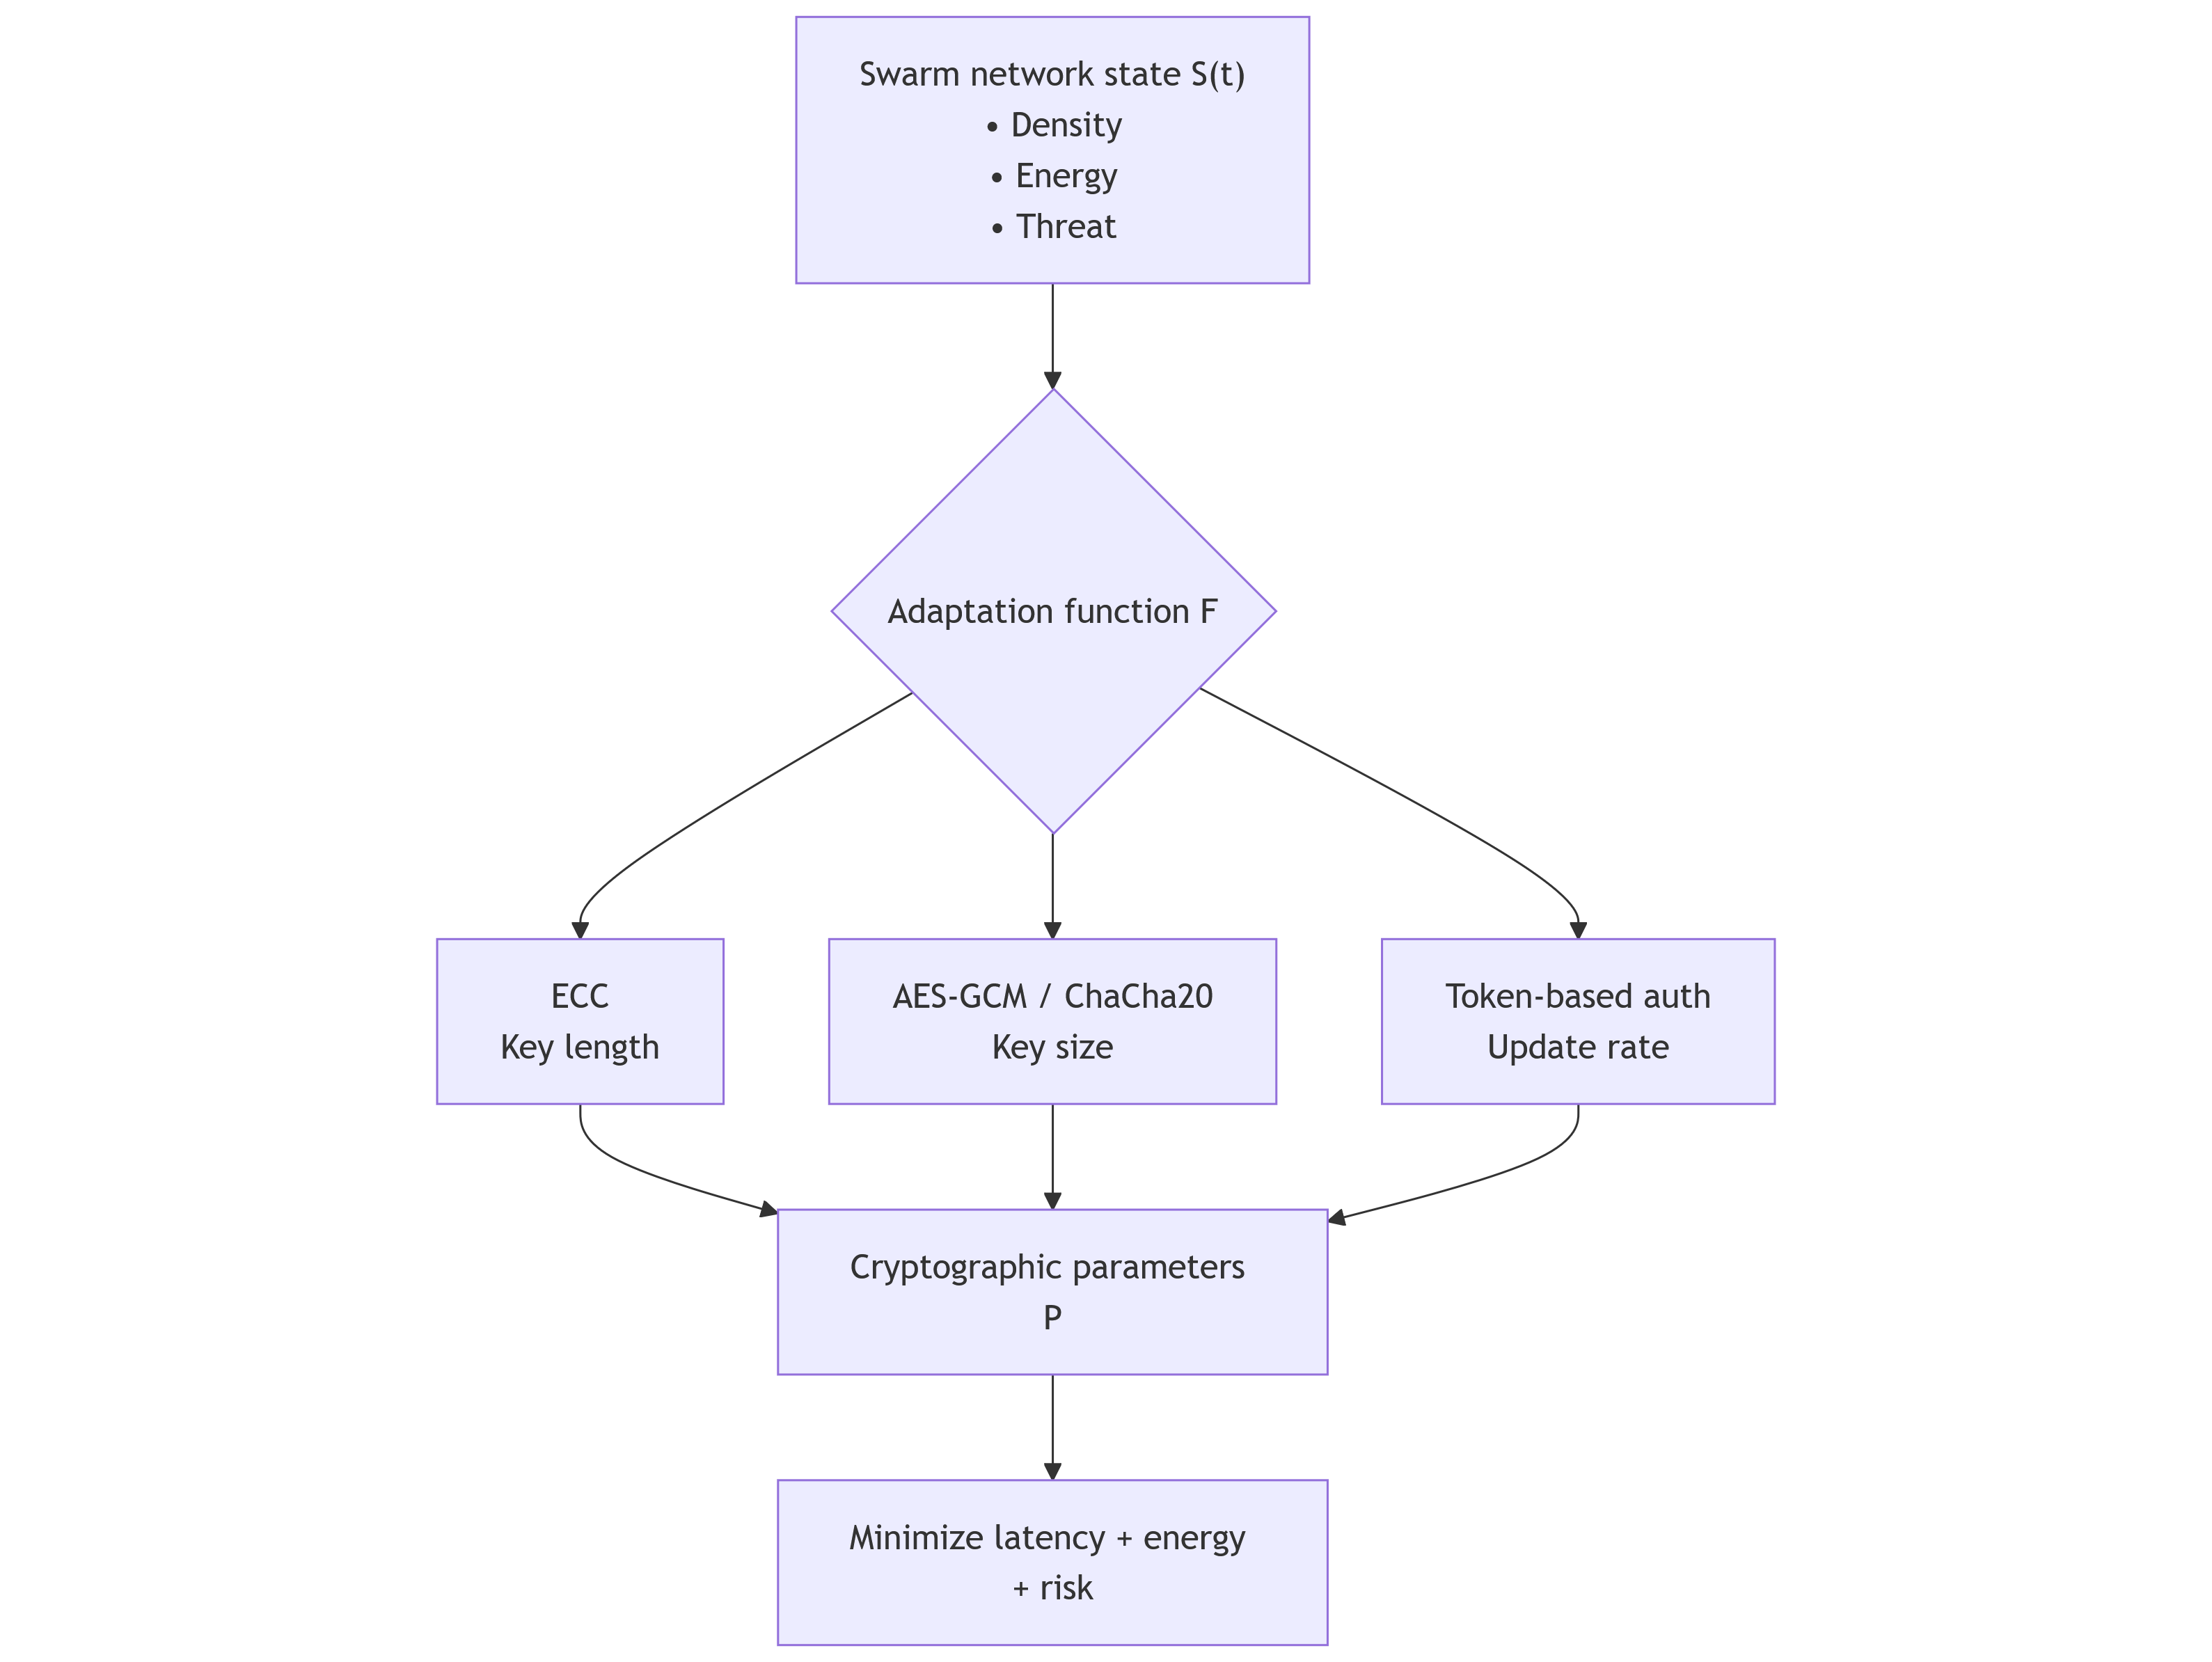
\includegraphics[width=0.9\textwidth]{figs/adaptive_crypto_framework}
\caption{Conceptual model of adaptive cryptographic selection based on swarm state.}
\label{fig:adaptive_crypto}
\end{figure}

Figure~\ref{fig:adaptive_crypto} summarizes this idea: observed swarm state is mapped to a cryptographic configuration that balances latency, energy use, and security level instead of fixing one operating mode for the entire mission.

\section{Decentralized Trust Mechanisms}
\label{sec:decentralized_trust}

To eliminate single points of failure, several studies extend swarm security with blockchain or distributed trust mechanisms. Sun and Shao~\cite{sunResearchDataSecurityEmergency2022} propose a blockchain-based communication scheme for heterogeneous emergency-response swarms, while Pacheco et al.~\cite{pachecoSecuringFederatedLearning2024} use blockchain to secure federated learning in robot swarms. Related trustless-agreement work similarly explores how robot collectives can provide distributed evidence for external decisions~\cite{pachecoSwarmOracleTrustless2025}. These works emphasize auditability and tamper resistance, but they also indicate a heavier protocol stack than the lightweight data-plane mechanisms discussed in the previous section.

Kohli et al.~\cite{kohliSwarmNetFirmwareAttestation2024} address trust from a different angle with \textit{Swarm-Net}, a firmware-attestation framework for IoT swarms based on graph neural networks and volatile-memory fingerprints. Adjacent adversarial-IoT and swarm-malware detection work reinforces the need to treat endpoint trust and runtime anomaly detection as separate but complementary layers~\cite{bommanaAddressingAdversarialAttacks2025,hanifOrchestratingMLSwarmMalware2025}. This work is relevant because it focuses on node integrity rather than message protection, illustrating that secure swarm systems require both trustworthy endpoints and secure channels.

Collectively, these studies reveal a persistent trade-off. Stronger decentralized trust mechanisms improve system assurance, but they are often too heavy for fast control loops or resource-constrained agents. Lightweight cryptographic approaches scale better, but they do not by themselves provide collective agreement or system-wide attestation.

\section{Adaptive Security Frameworks}
\label{sec:adaptive_security}

The reviewed literature suggests that secure swarm communication must combine three properties: lightweight runtime protection, decentralized operation, and adaptation to mission context. Existing works typically emphasize only one or two of these properties at a time. Connectivity-oriented designs prioritize resilience, lightweight schemes prioritize efficiency, and blockchain-style approaches prioritize trust.

Context-dependent security has been explored in adjacent IoT settings. Phalaagae et al.~\cite{phalaagaeEnergyEfficientAuthenticationCluster2024} show in clustered wireless sensor environments that authentication choices can be tuned to deployment constraints. Energy-aware encryption and zero-energy IoT discussions point in the same direction: protection mechanisms must be selected with the device power envelope in mind~\cite{khashanSmartEnergyEfficientEncryption2024,abbasTowardsZeroenergyNavigating2024}. In this thesis, that work is used as an adjacent-domain motivation for adaptive security rather than as direct swarm-robotics evidence.

For swarm robotics, this motivates an adaptive framework in which network density, remaining energy, packet loss, and threat estimates influence the choice of key length, cipher, authentication mode, and key-rotation policy. Such a framework does not replace the underlying primitives; instead, it orchestrates them according to mission state.

\section{Gap Analysis}
\label{sec:gap_analysis}

Within the reviewed corpus, three practical gaps remain most relevant to the present thesis. \textit{Static protocol configuration}: many lightweight schemes are evaluated with fixed security parameters even though mission conditions vary over time. \textit{Fragmented security layers}: communication resilience, trust, and message protection are often analyzed separately. \textit{Limited executable comparison}: adaptive ideas are frequently motivated conceptually, but common benchmark comparisons between stronger static, lighter static, and adaptive profiles are still rare in the selected literature.

These observations justify a narrower thesis contribution: an adaptive lightweight framework with retained formal reasoning and an executable benchmark for pairwise operating-mode comparison. They do not, by themselves, establish that the proposed benchmark is a complete swarm-security evaluation; that limitation is addressed explicitly in the later chapters.

\chapter{Theoretical Foundations and Methodology}
\label{chap:methodology}

\section{Formal Model of Swarm Networks}
\label{sec:formal_model}

A swarm network is represented as a dynamic graph $G(V,E,t)$ evolving over time. The set of vertices corresponds to swarm agents:
\begin{equation}
V = \{v_1, v_2, \ldots, v_n\},
\label{eq:vertices}
\end{equation}
where $n$ denotes the swarm size, which may change as nodes join or leave the system.

The set of edges $E(t) \subseteq V \times V$ models communication links at time $t$: an edge $(v_i, v_j) \in E(t)$ exists when agents are within wireless range and can exchange messages. The dynamic nature of the graph reflects robot mobility, environmental obstacles, and node failures.

Each vertex $v_i$ is characterized by a state $s_i(t)$ comprising:
\begin{itemize}
  \item position $p_i(t) \in \mathbb{R}^3$;
  \item velocity $\dot{p}_i(t)$;
  \item energy level $e_i(t) \in [0, E_{\max}]$;
  \item computational resources, including processor clock frequency $f_i$ and memory capacity $m_i$;
  \item cryptographic parameters, including the current encryption key $k_i(t)$ and key length $l_i(t)$.
\end{itemize}

The global swarm state
\begin{equation}
S(t) = \{s_1(t), s_2(t), \ldots, s_n(t)\},
\label{eq:global_state}
\end{equation}
aggregates the individual node states.

Communication channels are modeled as random variables reflecting wireless conditions. The bandwidth of channel $(v_i, v_j)$ depends on inter-node distance $d_{ij}(t) = \|p_i(t) - p_j(t)\|$ and environmental noise. Channel latency $\tau_{ij}(t)$ includes propagation delay
\begin{equation}
\tau_{\text{prop}} = \frac{d_{ij}}{c},
\label{eq:prop_delay}
\end{equation}
where $c$ is the speed of light, plus processing delay $\tau_{\text{proc}}$. Packet losses $L_{ij}(t)$ model congestion, interference, or malicious jamming.

Resource constraints formalize the embedded setting: processing power is limited, memory is bounded, and depletion of $e_i(t)$ renders a node inoperable. Transmission energy consumption is proportional to the square of distance, $E_{\text{tx}} \propto d_{ij}^2$, while cryptographic operations consume energy proportional to algorithmic complexity:
\begin{equation}
E_{\text{crypto}} = \alpha \cdot C_{\text{ops}},
\label{eq:crypto_energy}
\end{equation}
where $C_{\text{ops}}$ denotes the number of cryptographic operations and $\alpha$ is the energy cost per operation.

The model supports performance analysis through throughput, end-to-end latency, and energy efficiency. Cryptographic overhead is measured by additional latency $\Delta \tau_{\text{crypto}}$ and energy consumption $\Delta E_{\text{crypto}}$ relative to unsecured transmission. The adaptive framework seeks to minimize these costs while maintaining the required security level.

A cost function $J(S(t), P(t))$ evaluates the trade-off between performance and security, where $P(t)$ denotes the vector of cryptographic parameters for all nodes. The optimization problem is defined as
\[
\min_{P(t)} J(S(t), P(t))
\]
subject to energy and latency constraints $e_i(t) > E_{\min}$ and $\tau_{ij}(t) < \tau_{\max}$. The solution determines the optimal encryption parameters for the current swarm state.
In the later benchmark prototype, this optimization view is approximated by a threshold-based selector rather than solved directly.

\section{Threat Model and Security Requirements}
\label{sec:threat_model}

The adversarial model classifies the capabilities of an attacker. A \emph{passive adversary} eavesdrops on communications, an \emph{active adversary} modifies or injects messages, and a \emph{compromised node} scenario assumes access to keys and memory. The Dolev--Yao model assumes network control with perfect cryptographic primitives; extended models account for computationally bounded adversaries and implementation-level weaknesses.

Attack types relevant to swarms include eavesdropping, message tampering, impersonation, replay, Sybil, wormhole, and denial-of-service attacks.

Confidentiality requirements protect message contents from unauthorized access. In the present thesis, confidentiality at the data-plane level is operationalized through AEAD schemes with unique nonces per encryption. This is a design requirement for the prototype rather than a claim derived from the swarm-robotics literature itself.

Authentication requirements ensure sender authenticity and message integrity. EUF-CMA (Existential Unforgeability under Chosen-Message Attack) guarantees that an adversary cannot forge a valid signature for a new message after observing chosen-message queries. Digital signature schemes such as ECDSA and Schnorr provide EUF-CMA under standard cryptographic assumptions, while MACs such as HMAC and Poly1305 provide symmetric-key authentication~\cite{nistFips198HMAC,rfc8439}.

Data integrity prevents undetected message modification. Cryptographic hash functions such as SHA-256 and Blake2 produce fixed-length digests; authenticated encryption schemes such as AES-GCM and ChaCha20-Poly1305 combine confidentiality and integrity in one step~\cite{nistSP80038DGCM,rfc8439}.

Additional security properties can strengthen swarm systems beyond the current prototype, especially resilience to node compromise and stronger protection of past sessions through rekeying. Swarm missions differ in criticality, but the prototype evaluated later in the thesis focuses on a narrower question: how switching between stronger and lighter communication profiles affects performance and model-based efficiency under constrained execution. In this thesis, confidentiality, authentication, integrity, and compromise containment are treated as the core security requirements for the executable benchmark, as summarized in Table~\ref{tab:security_requirements}.

\renewcommand{\arraystretch}{1.1}
\begin{longtable}{|>{\raggedright\arraybackslash}p{0.27\textwidth}|>{\raggedright\arraybackslash}p{0.23\textwidth}|>{\raggedright\arraybackslash}p{0.22\textwidth}|>{\raggedright\arraybackslash}p{0.16\textwidth}|}
\caption{Security Requirements and Corresponding Cryptographic Mechanisms}
\label{tab:security_requirements} \\
\hline
\textbf{Security Requirement} & \textbf{Definition} & \textbf{Mechanism} & \textbf{Swarm Application} \\
\hline
\endfirsthead
\caption[]{Security Requirements and Corresponding Cryptographic Mechanisms (continued)} \\
\hline
\textbf{Security Requirement} & \textbf{Definition} & \textbf{Mechanism} & \textbf{Swarm Application} \\
\hline
\endhead
Confidentiality (IND-CPA) &
Ciphertext is indistinguishable from random data &
AES-GCM, ChaCha20, ECC-based encryption &
Protection of sensor data and coordinates \\
\hline
Authentication (EUF-CMA-style goal) &
Runtime authenticators cannot be forged without the relevant secret &
HMAC, token-based hash chains, digital signatures for control messages &
Verification of packet origin and trusted updates \\
\hline
Data integrity &
Unauthorized modifications are detected &
Hash functions, MACs, authenticated encryption &
Prevention of message tampering \\
\hline
Compromise containment &
Rekeying limits the impact of disclosed session state &
Per-epoch ECDH and periodic key refresh &
Damage reduction after local compromise \\
\hline
\end{longtable}

\section{Mathematical Toolkit}
\label{sec:math_toolkit}

Computational complexity theory classifies algorithms according to asymptotic resource requirements. Time complexity $T(n)$ denotes the number of elementary operations as a function of input size $n$, and space complexity $S(n)$ denotes memory usage. Common classes include:
\begin{itemize}
  \item $O(1)$ --- constant;
  \item $O(\log n)$ --- logarithmic;
  \item $O(n)$ --- linear;
  \item $O(n \log n)$ --- linearithmic;
  \item $O(n^2)$ --- quadratic.
\end{itemize}
Cryptographic operations have characteristic cost patterns:
\begin{itemize}
  \item symmetric block encryption --- $O(1)$ for a fixed block size;
  \item hashing a message of length $n$ --- $O(n)$;
  \item elliptic-curve scalar multiplication --- substantially more expensive than a single symmetric-message operation on constrained platforms;
  \item modular exponentiation --- typically heavier than lightweight symmetric protection in the same environment.
\end{itemize}
For swarm systems, swarm size $n$ is critical; protocols with quadratic communication or synchronization cost become progressively less attractive as the number of participating nodes grows.

Game-theoretic models analyze interactions between legitimate agents and an adversary. In a simple security game, the defender selects a cryptographic parameter $p \in P$, the adversary selects an attack $a \in A$, and the payoff $U(p,a)$ is the attack success probability.
In a Stackelberg game, the defender commits to parameters first and the adversary responds, so the adaptation function $F$ selects parameters that increase the cost of a successful attack.

Information-theoretic security analysis evaluates fundamental limits of information protection. Shannon entropy is defined as
\begin{equation}
H(X) = - \sum_x p(x)\log p(x).
\label{eq:shannon_entropy}
\end{equation}
It measures the uncertainty of a random variable $X$. Perfect secrecy is defined by $H(M \mid C) = H(M)$, meaning ciphertext $C$ conveys no information about message $M$. Practical schemes target computational security; mutual information
\[
I(M;C) = H(M) - H(M \mid C)
\]
quantifies information leakage, and minimizing $I(M;C)$ is a protocol design objective. Secure channel capacity is expressed as
\begin{equation}
C_s = C - \varepsilon,
\label{eq:secure_capacity}
\end{equation}
where $C$ is channel capacity and $\varepsilon$ denotes leakage to the adversary.

Asymptotic performance analysis characterizes protocol scalability. Communication complexity is the number of bits transmitted between nodes. For key exchange, ECDH requires one round and communication cost proportional to the exchanged public-key material. For authentication of many messages, aggregation can reduce repeated verification overhead, although the executable benchmark in this thesis does not implement batched verification.
\begin{itemize}
  \item an $O(n)$ protocol scales linearly with swarm size;
  \item an $O(n^2)$ protocol imposes pairwise cost growth that can quickly dominate runtime and synchronization overhead.
\end{itemize}
The broader adaptive framework therefore aims to avoid unnecessary pairwise coordination work, even though the benchmarked prototype later in the thesis is intentionally restricted to a pairwise data path.

Probabilistic analysis models random failures and attacks. Let the probability of node compromise be $p_c$; then the number of compromised nodes follows
\[
N_c \sim \mathrm{Binomial}(n, p_c).
\]
Under threshold cryptography, a secret is reconstructible from $t$ out of $n$ nodes; the probability of secret loss is
\begin{equation}
P_{\text{fail}} = \sum_{k=t}^{n} \binom{n}{k} p_c^k (1-p_c)^{n-k}.
\label{eq:threshold_failure}
\end{equation}
Choosing $t$ is a security-availability trade-off. Message delay can be modeled by an exponential distribution $\tau \sim \mathrm{Exp}(\lambda)$, yielding
\[
P(\tau > \tau_{\max}) = e^{-\lambda \tau_{\max}}.
\]
Shorter keys reduce $\tau$ but increase $P_{\text{break}}$, whereas longer keys improve security at the cost of higher delay.

Optimization methods cast protocol design as a mathematical programming problem. A typical objective minimizes a weighted sum of delay, energy, and risk:
\begin{equation}
J = w_1 \tau + w_2 E + w_3 R,
\label{eq:objective}
\end{equation}
where $w_i$ are weighting coefficients. Constraints include node energy $e_i > E_{\min}$, latency $\tau < \tau_{\max}$, and security risk $R < R_{\max}$. Decision variables include key length $l$, rotation frequency $f_{\mathrm{rot}}$, the data-plane cipher $a \in \{\mathrm{AES}, \mathrm{ChaCha}\}$, and the runtime authentication mode $m_{\mathrm{auth}}$. In the benchmarked prototype, $m_{\mathrm{auth}}$ is either HMAC-SHA256 or a sequence-bound hash token. If $J$ is convex, the optimum can be found efficiently; otherwise, heuristic methods may be required.

This toolkit provides the basis for the performance bounds and security proofs derived later (Fig.~\ref{fig:math_foundations}).

\begin{figure}[H]
\centering
% Export the Mermaid diagram (SVG/PDF/PNG) and place it in figs/ if you want LaTeX compilation.
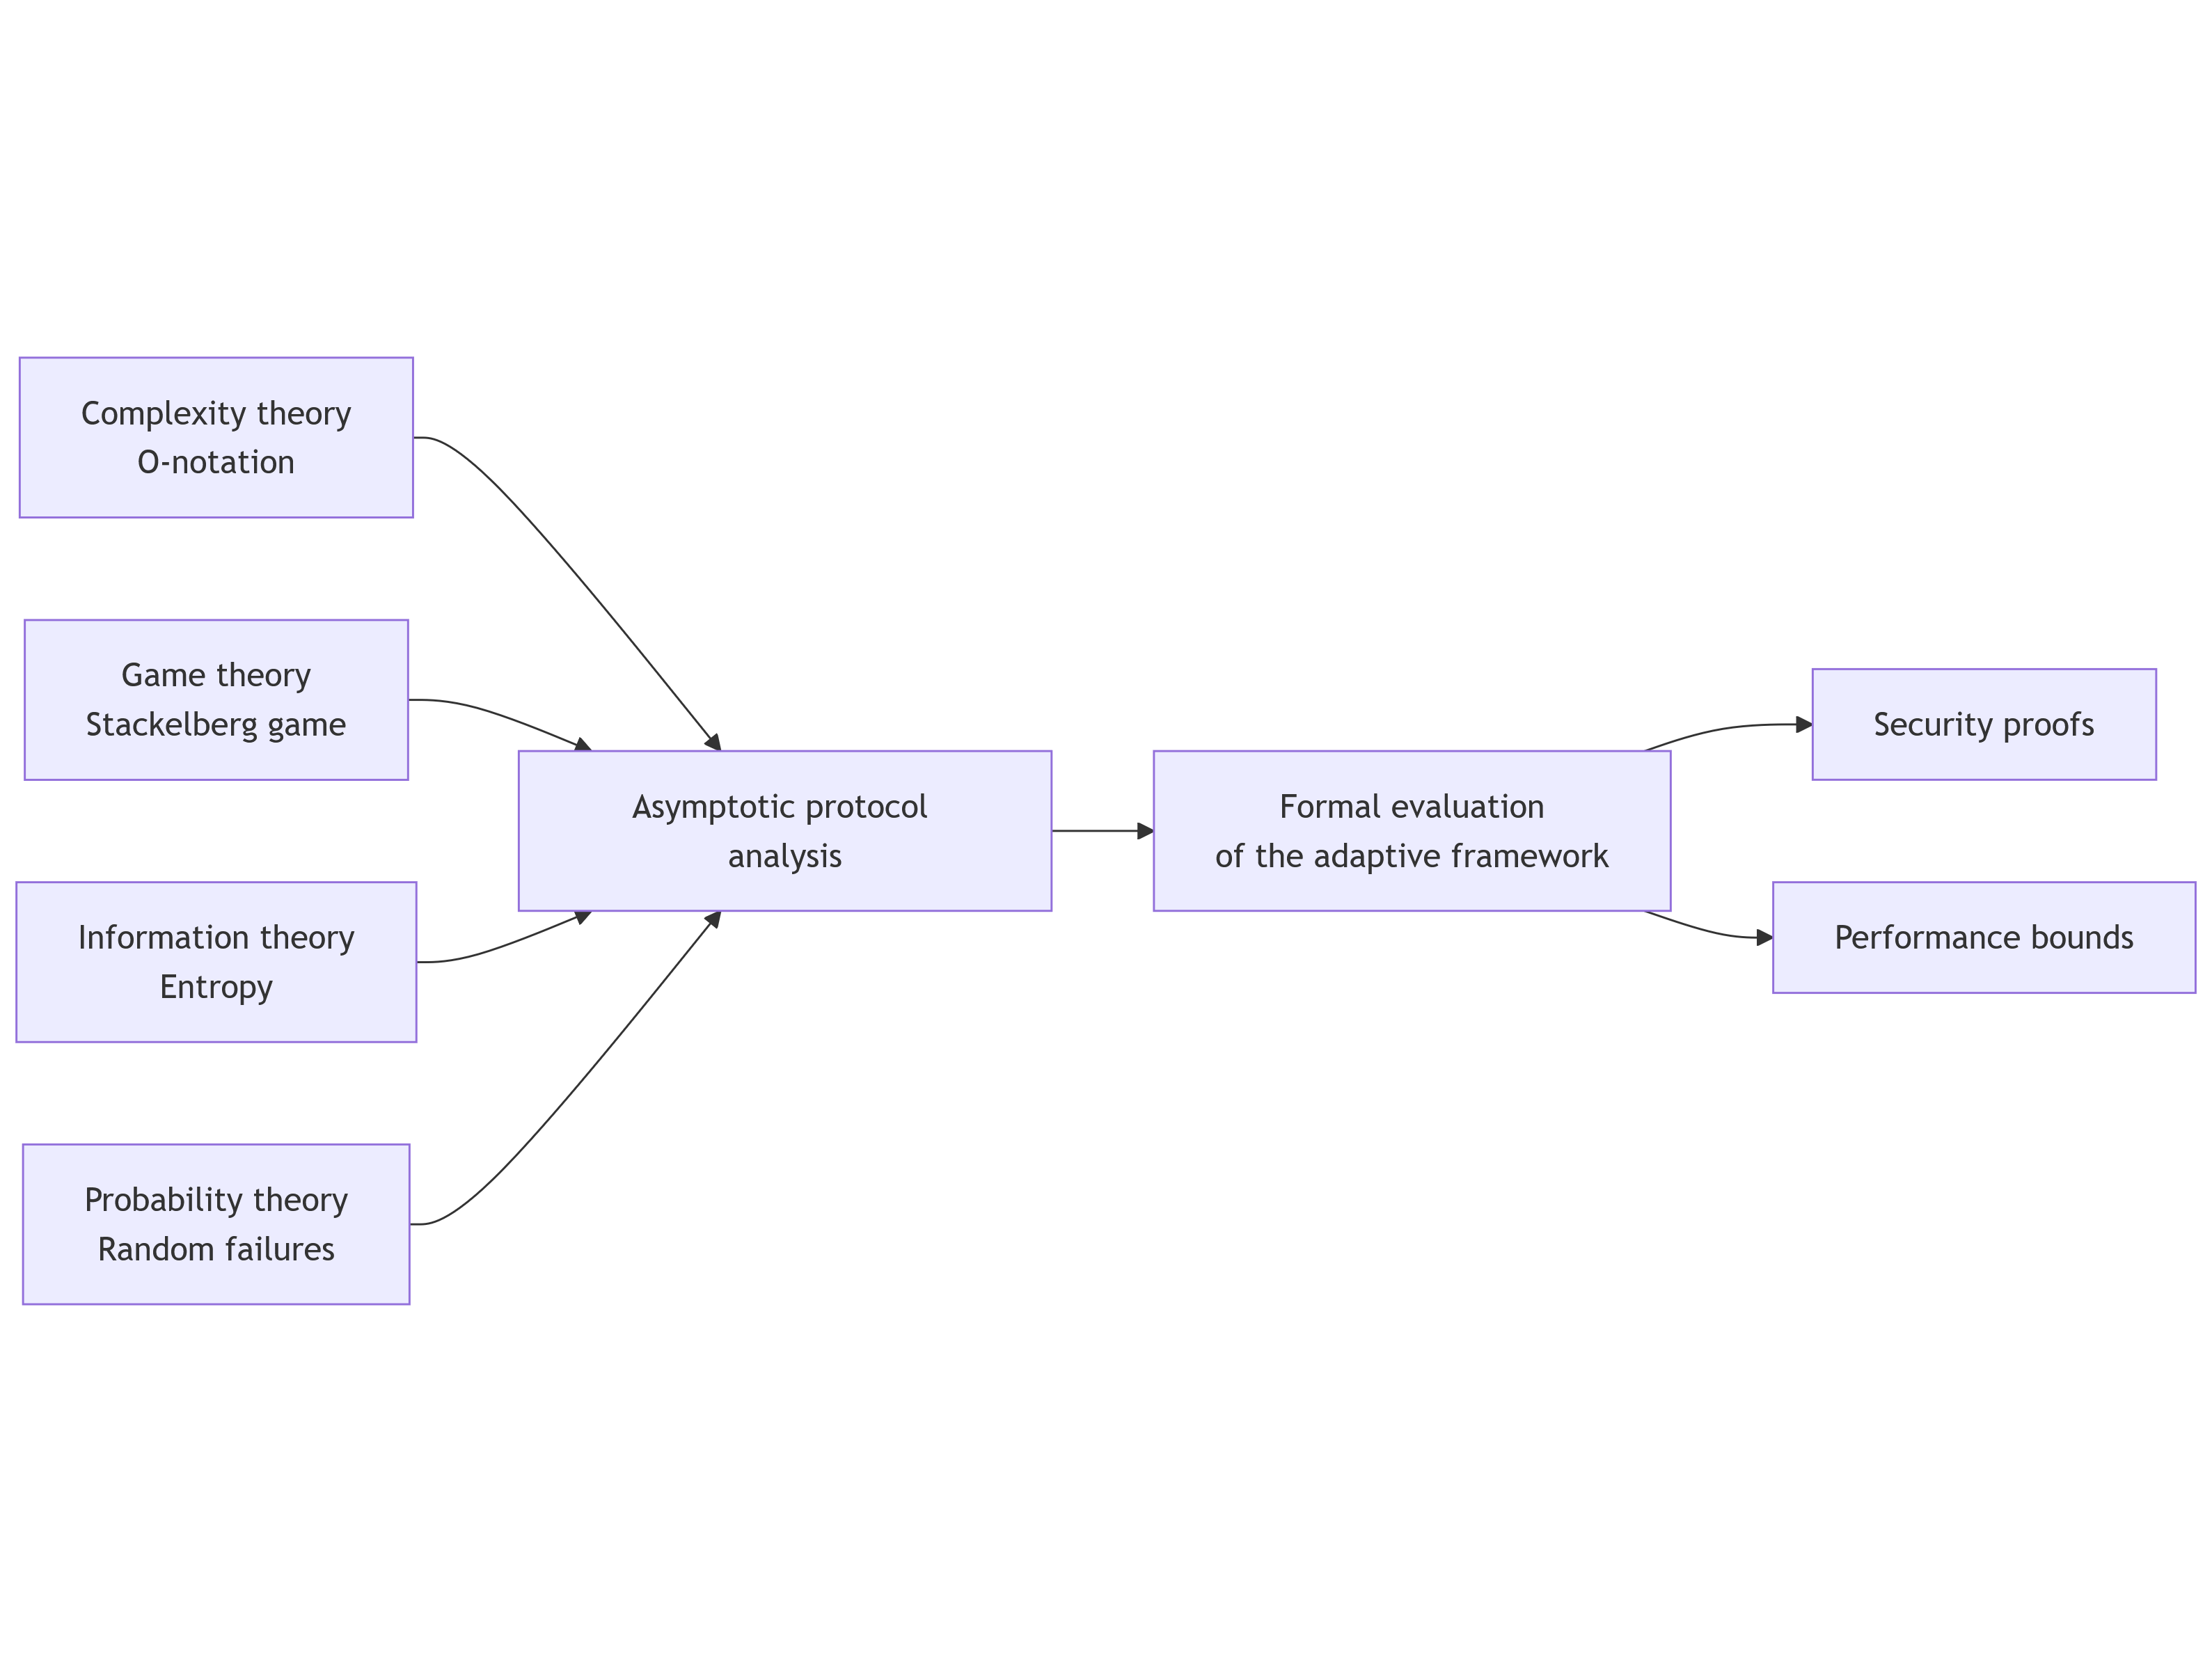
\includegraphics[width=\textwidth]{figs/math_foundations.png}
\caption{Mathematical foundations for analyzing the adaptive framework.}
\label{fig:math_foundations}
\end{figure}

The diagram visualizes the integration of theoretical disciplines used later in the thesis.


\section{Methodology Overview}
\label{sec:methodology_overview}

The research methodology is structured into sequential stages. \textbf{Stage 1: literature consolidation} reviews ECC-based key exchange, symmetric encryption with pre-shared keys, and token-based authentication, then summarizes their complexity, overhead, and security trade-offs~\cite{adeniyiSystematicReviewECC2024,kumarComprehensiveSurveyAuthenticationIoT2022}.

\textbf{Stage 2: theoretical framework development} defines the swarm graph, the threat model, the security requirements, and the adaptation function $F$, together with the optimization objective $J(S,P)$.

\textbf{Stage 3: complexity analysis of baseline protocols} derives relative computational bounds for each protocol. For ECC--ECDH, scalar multiplication is treated as the dominant setup cost, while communication cost is proportional to the exchanged public-key material. For AES-GCM:
\begin{itemize}
  \item block encryption is $O(1)$ per block;
  \item authentication is $O(n)$ for a message consisting of $n$ blocks.
\end{itemize}
For hash-chain tokens, generation of a chain of length $L$ costs $O(L \cdot h)$ and token verification costs $O(h)$. Communication overhead is summarized through message sizes, and protocols linear in the number of nodes are preferred for large swarms.

\textbf{Stage 4: retained formal security analysis} identifies vulnerabilities and attack vectors, then connects the data-plane confidentiality and authentication goals to standard assumptions about the employed primitives. The purpose of this stage is to bound the claims made later in the thesis, not to present a full end-to-end proof of the adaptive benchmark implementation.

\textbf{Stage 5: adaptive framework design} develops the adaptation function $F: S(t) \rightarrow P(t)$. At the architectural level, network density is expressed as
\begin{equation}
\rho = \frac{n}{A},
\label{eq:density}
\end{equation}
where $A$ is the coverage area. The average energy level is
\begin{equation}
\bar{e} = \frac{1}{n}\sum e_i.
\label{eq:avg_energy}
\end{equation}
Threat level $\theta \in [0,1]$ is estimated from anomaly detection. Tuning parameters include key length $l \in \{192,256\}$ for the AES-based profiles used in the benchmark, a ChaCha20-Poly1305 lightweight profile, a scenario-fixed rekey interval, and the runtime authentication mode. The prototype uses HMAC-SHA256 for the AES-based profiles and a sequence-bound hash token for the lightweight profile. The cost function is defined as
\begin{equation}
J = \alpha \tau(l,a,m_{\mathrm{auth}}) + \beta E_{\mathrm{crypto}}(l,a,m_{\mathrm{auth}}) + \gamma R(\theta,l,m_{\mathrm{auth}}),
\label{eq:cost_function}
\end{equation}
where $\tau$ is latency, $E_{\mathrm{crypto}}$ is a platform-dependent energy term, and $R$ is a symbolic residual-risk term. In the executable prototype, the decision procedure is simplified to:
\[
\text{if } \theta \geq \theta_{\mathrm{high}} \text{ then select heavy profile;}
\]
\[
\text{else if } \bar{e} \leq E_{\mathrm{crit}} \text{ then select lightweight profile;}
\]
\[
\text{else select balanced profile.}
\]

\textbf{Stage 6: protocol specification} describes the initialization, operational, and adaptation phases of the prototype actually evaluated later: agents establish pairwise keys with X25519-based exchange, derive symmetric material with HKDF, and switch among heavy, balanced, and lightweight data-plane profiles according to scripted threat and energy inputs.
\begin{equation}
P(t) = F(S(t)),
\label{eq:adaptation}
\end{equation}
The broader density-aware and consensus-aware design remains a conceptual extension rather than a benchmarked implementation artifact.

\textbf{Stage 7: practical benchmark evaluation} runs the implemented protocol under constrained CPU and memory budgets, compares static-heavy, static-balanced, static-lightweight, and adaptive modes, and records measured latency, throughput, switching behavior, and normalized energy proxies.

\textbf{Stage 8: design guidelines formulation} translates the findings into practical recommendations for scenario-specific parameterization, primitive selection, and secure deployment.

The methodology provides a path from formal modeling to design, implementation, and benchmark-based evaluation of an adaptive framework, while keeping the security--performance trade-off explicit.

\chapter{Comparative Analysis of Baseline Protocols}
\label{chap:comparison}

\section{Analysis of ECC-Based Key Exchange}
\label{sec:ecc_key_exchange}

Elliptic Curve Diffie--Hellman (ECDH) establishes a shared secret without prior key distribution and is the key-establishment primitive used throughout this thesis. The prototype uses the X25519 function standardized for Diffie--Hellman use over Curve25519~\cite{rfc7748}. Agent $v_i$ generates a private key $d_i$, chosen uniformly at random from the interval $[1, n-1]$, where $n$ denotes the order of the elliptic-curve group. The corresponding public key is computed as
\begin{equation}
Q_i = d_i \cdot G,
\label{eq:ecdh_public_key}
\end{equation}
where $G$ is the base point of the curve and $\cdot$ denotes elliptic-curve scalar multiplication.
Agent $v_j$ analogously generates $(d_j, Q_j)$. During public key exchange, $v_i$ sends $Q_i$ to $v_j$, and $v_j$ sends $Q_j$ to $v_i$. The shared secret is then computed as
\[
K = d_i \cdot Q_j \quad \text{by } v_i, \qquad
K = d_j \cdot Q_i \quad \text{by } v_j.
\]
Due to commutativity, both computations yield the identical value $K = d_i d_j \cdot G$.

The computational cost of ECDH is dominated by elliptic-curve scalar multiplication, so it is expensive relative to symmetric cryptography but acceptable for periodic setup and rekeying. Memory and energy costs scale with the number of neighbors, which is why ECDH is used for session establishment rather than per-message protection. Its security rests on the hardness of ECDLP; forward secrecy is obtained only when the exchanged key material is ephemeral or refreshed per session/epoch. Authenticated, group, and threshold variants are useful for specific deployment constraints, but they do not change ECDH's role as the setup primitive.


\section{Symmetric Encryption Schemes}
\label{sec:symmetric_encryption}

AES-GCM and ChaCha20-Poly1305 are the symmetric primitives used for bulk payload protection once a shared secret exists. AES is standardized with 128-, 192-, and 256-bit key sizes~\cite{nistFips197AES}, and GCM is the NIST-specified authenticated-encryption mode used by the heavy and balanced profiles~\cite{nistSP80038DGCM}. ChaCha20-Poly1305 is specified for IETF protocols and is a practical software-oriented AEAD alternative~\cite{rfc8439}. AES-GCM is preferred when hardware acceleration is available; ChaCha20-Poly1305 is preferred on software-only microcontrollers. Both provide confidentiality and integrity with a 96-bit nonce and a 128-bit tag. In the thesis architecture, these ciphers are paired with ECDH-derived session keys and periodic rotation, which keeps asymmetric operations off the per-message path.


\section{Token-Based Authentication}
\label{sec:token_auth}

Hash-chain schemes provide lightweight authentication through a precomputed sequence of hash values. An agent generates an initial random seed $s_0$ and iteratively applies a cryptographic hash function $H$:
\begin{equation}
s_1 = H(s_0),\; s_2 = H(s_1),\; \ldots,\; s_L = H(s_{L-1}).
\label{eq:hash_chain}
\end{equation}
The final hash $s_L$ is published as a commitment, while the tokens $s_{L-1}, s_{L-2}, \ldots, s_0$ are used sequentially for authentication. Upon receiving a token $s_i$, the verifier computes $H(s_i)$ and compares it with the previously accepted token $s_{i+1}$ or with the commitment; a match confirms authenticity. The one-wayness of the hash function prevents efficient recovery of previous chain elements from later ones, but this property should not be conflated with full channel-level forward secrecy. Runtime cost is low because token generation and token verification require only hash evaluations, while communication overhead is limited to the transmitted token itself~\cite{manikandanASMTPAnonymousSecureMessaging2024}.

The Anonymous Secure Messaging Token-Based Protocol (ASMTP) extends hash-chain authentication for UAV swarms by attaching a token to each message instead of an explicit identifier. The receiver verifies the token without learning the sender’s identity, which makes the scheme attractive for lightweight telemetry and control traffic. Its main limitation is synchronization: packet loss can desynchronize sender and receiver, so the protocol must either include the token index or periodically reinitialize the chain. The prototype in this thesis uses a simpler sequence-bound hash token inspired by this lightweight-authentication family, not the full ASMTP disclosure protocol. The additional latency and energy of token-style checks are negligible compared to radio transmission, while communication overhead is just the token itself.

Synchronization issues represent a practical challenge for hash-chain schemes. Packet loss may desynchronize the receiver, which expects token $s_i$ but receives $s_{i-k}$. One solution is to include the index $i$ in the message, enabling verification by computing
\begin{equation}
H^{k}(s_{i-k}) = s_i,
\label{eq:hash_resync}
\end{equation}
where $H^{k}$ denotes $k$ successive applications of the hash function. The cost of this approach is partial disclosure of the chain position and potential predictability of future indices. Alternative solutions include maintaining backup chains or periodically regenerating chains after exhaustion or compromise.


\section{Complexity and Performance Comparison}
\label{sec:complexity_comparison}

Comparative tables integrate the main trade-offs across the three protocol categories. ECDH is the costliest primitive but provides key establishment and forward secrecy; AES-GCM and ChaCha20-Poly1305 are efficient for payload protection once keys exist; and hash-chain authentication is the lightest option for frequent verification. HMAC remains the conventional keyed-hash mechanism for additional message authentication in the heavy and balanced profiles~\cite{nistFips198HMAC}. The thesis therefore adopts a hybrid stack and applies each primitive only where it is most appropriate.

\begin{landscape}
\begin{table}[H]
\centering
\small
\setlength{\tabcolsep}{5pt}
\caption{Qualitative comparison of baseline protocol roles in the proposed architecture}
\label{tab:protocol_comparison}
\renewcommand{\arraystretch}{1.2}
\begin{tabularx}{\linewidth}{|l|c|c|c|>{\raggedright\arraybackslash}X|>{\raggedright\arraybackslash}X|}
\hline
\textbf{Protocol} &
\textbf{Setup Cost} &
\textbf{Runtime Cost} &
\textbf{Overhead} &
\textbf{Primary Role} &
\textbf{Main Limitation} \\
\hline
ECDH-256 &
High &
Not used per message &
Public-key exchange &
Session establishment and forward secrecy &
Expensive to repeat frequently in dense networks \\
\hline
AES-128-GCM &
Medium &
Low with hardware support &
Nonce + tag &
Authenticated payload protection &
Benefits strongly from hardware acceleration \\
\hline
AES-256-GCM &
Medium--high &
Higher than AES-128 &
Nonce + tag &
Maximum-strength authenticated payload protection &
Higher compute cost than lightweight modes \\
\hline
ChaCha20-Poly1305 &
Low &
Low on software-only targets &
Nonce + tag &
Software-oriented authenticated encryption &
Still depends on robust key management \\
\hline
Hash-chain (SHA-256) &
Low &
Very low verification cost &
Token per message &
Lightweight authentication for frequent traffic &
Sensitive to synchronization loss \\
\hline
\end{tabularx}
\end{table}
\end{landscape}



The table highlights the same conclusion in compact form: no single protocol dominates across all dimensions. ECC is essential for secure key establishment without pre-existing infrastructure; symmetric encryption provides efficient confidentiality once keys are available; and hash-chain schemes offer ultra-lightweight authentication. The optimal strategy is therefore a hybrid approach that combines these primitives and selects them adaptively based on current security requirements, network conditions, and available resources rather than relying on one fixed profile.

\chapter{Design of the Adaptive Encryption Framework}
\label{chap:adaptive_framework}

\section{Design of the Adaptation Function}
\label{sec:adaptation_function}

The adaptation function $F: S(t) \rightarrow P(t)$ maps the observed communication state to a runtime cryptographic profile. In the broader architectural model, the state vector may include density, energy, packet loss, and threat level. For the executable prototype evaluated in this thesis, the effective switching rule is narrower and uses only threat and energy as direct inputs. This distinction is important: the chapter presents the architectural motivation first, then fixes the smaller state space that is actually implemented and benchmarked.

At the conceptual level, density is defined as
\begin{equation}
\rho(t) = \frac{n(t)}{A(t)},
\label{eq:density_time}
\end{equation}
where $n(t)$ is the number of active nodes and $A(t)$ is the covered area. The average energy level is
\begin{equation}
\bar{e}(t) = \frac{1}{n}\sum_{i=1}^{n} e_i(t),
\label{eq:avg_energy_time}
\end{equation}
and threat level is represented by $\theta(t) \in [0,1]$. In a full swarm deployment, packet loss $\lambda(t)$ and neighborhood dynamics would also inform profile selection. In the benchmark prototype, however, profile selection is reduced to threshold checks over $\bar{e}(t)$ and $\theta(t)$.

The benchmarked parameter vector is discrete:
\[
P(t) \in \{\text{heavy}, \text{balanced}, \text{lightweight}\}.
\]
These three profiles are defined as follows.
\begin{itemize}
  \item \textbf{Heavy}: AES-256-GCM for encryption and HMAC-SHA256 for additional data-plane authentication.
  \item \textbf{Balanced}: AES-192-GCM for encryption and HMAC-SHA256 for additional data-plane authentication.
  \item \textbf{Lightweight}: ChaCha20-Poly1305 for encryption and integrity, plus a sequence-bound hash token used as an inexpensive runtime authenticator.
\end{itemize}

The conceptual cost function remains
\begin{equation}
J = \alpha \cdot \tau(P) + \beta \cdot E(P) + \gamma \cdot R(S,P),
\label{eq:cost_function_adaptive}
\end{equation}
where $\tau(P)$ is latency, $E(P)$ is a platform-dependent energy term, and $R(S,P)$ is a residual-risk term. In this thesis, $J$ is used as a design lens rather than as a solved optimization problem. The practical benchmark does not claim to compute a globally optimal $P$; it validates that a threshold-based controller can switch among stronger and lighter profiles in a reproducible way.

The implemented decision rule is:
\begin{itemize}
  \item if $\theta \geq 0.8$, select the heavy profile;
  \item else if $\bar{e} \leq 0.2E_{\max}$, select the lightweight profile;
  \item else select the balanced profile.
\end{itemize}

Optimization-based and learned variants are possible extensions, but they are not implemented in the benchmark suite used in this work. The measured results later in the thesis therefore support claims about adaptive switching behavior, not about optimal profile selection.

\begin{figure}[H]
\centering
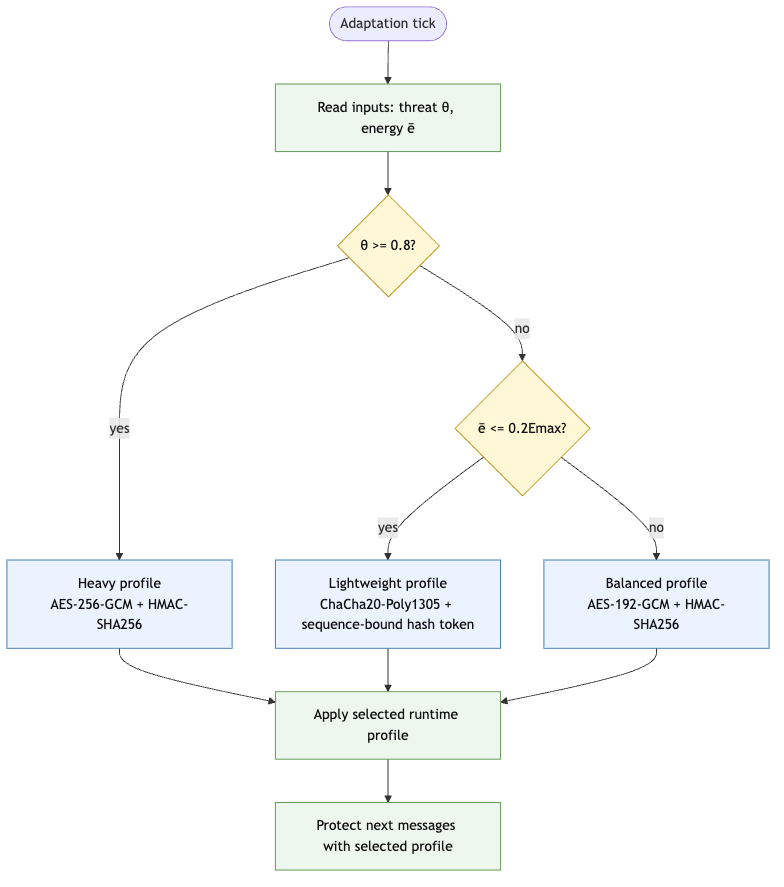
\includegraphics[width=\textwidth]{figs/adaptive_algorithm.png}
\caption{Adaptive cryptographic parameter selection algorithm.}
\label{fig:adaptive_algorithm}
\end{figure}

Figure~\ref{fig:adaptive_algorithm} should be read as an architectural diagram. The executable prototype instantiates its simplest branch: a threshold controller over threat and energy.

\section{Protocol Specification}
\label{sec:protocol_specification}

The protocol described in this thesis has two layers of scope. The first is the broader swarm-oriented architecture motivated by the literature. The second is the concrete pairwise prototype used in the practical evaluation. The practical evaluation validates only the second layer.

The \emph{initialization phase} of the prototype is pairwise. Peers are configured with a benchmark mode and a rekey interval, execute an X25519 key exchange, and derive epoch-specific material with HKDF-SHA256~\cite{rfc7748,rfc5869}. The resulting session keys are
\begin{equation}
k^{\mathrm{enc}}_{ij} = \mathrm{KDF}(K_{ij}, \text{``encryption''}),
\label{eq:kdf_enc}
\end{equation}
\begin{equation}
k^{\mathrm{mac}}_{ij} = \mathrm{KDF}(K_{ij}, \text{``authentication''}),
\label{eq:kdf_mac}
\end{equation}
where $K_{ij}$ is the X25519-derived shared secret. A fresh exchange is repeated on rekey events so that each epoch uses newly derived material. This supports compromise containment at the epoch level. The benchmark does not implement signed bootstrap announcements or signed configuration updates, so the practical evaluation should not be interpreted as validating control-plane authenticity.

The \emph{operational phase} protects each message with the currently selected runtime profile. For message transmission, the sender generates a nonce $N$ and encrypts plaintext $m$ as
\begin{equation}
c = \mathrm{Enc}\!\left(k^{\mathrm{enc}}_{ij}, N, m\right).
\label{eq:encrypt_msg}
\end{equation}
The transmitted packet format depends on the active profile.
\begin{itemize}
  \item In the heavy and balanced profiles, the packet carries $\{N, c, \sigma\}$ where $\sigma=\mathrm{MAC}(k^{\mathrm{mac}}_{ij}, N \Vert c)$.
  \item In the lightweight profile, the packet carries $\{N, c, h_i\}$ where $h_i$ is the sequence-bound hash token associated with the current epoch and message sequence number.
\end{itemize}
Upon reception, the receiver verifies the profile-appropriate authenticator, rejects already accepted sequence numbers within the current epoch, and decrypts only if verification succeeds.

The \emph{adaptation phase} is also pairwise in the prototype. At each adaptation interval, the sender reads the current threat and energy inputs from the active scenario, applies the threshold rule, and chooses one of the three runtime profiles. The benchmark does not implement gossip-based aggregation, leader election, or consensus-based synchronized switching across many nodes. Those mechanisms remain architectural extensions for a future multi-peer implementation.

The main loop can be summarized as follows:

\begin{lstlisting}
Initialization:
  Generate X25519 key pair
  Perform pairwise key exchange
  Derive epoch keys via HKDF
  Set initial profile P <- balanced

Operational loop:
  Every T_adapt seconds:
    Read current threat and energy inputs
    Compute P_new <- F(threat, energy)
    If P_new != P:
      Switch runtime profile: P <- P_new

  On sending message m:
    Generate nonce N
    Encrypt per selected profile
    Attach HMAC or hash token
    Transmit packet

  On receiving packet:
    Verify profile-appropriate authenticator
    If verification succeeds:
      Decrypt and process
    Else:
      Drop packet
\end{lstlisting}

This specification is intentionally narrower than a full swarm-control-plane protocol. It is, however, sufficient for the benchmarked claim of this thesis: a pairwise adaptive secure-communication prototype can be implemented, switched between profiles, and measured under constrained execution.

\section{Parameter Selection Algorithm}
\label{sec:parameter_selection}

For the executable benchmark, the input metrics of the selector are intentionally minimal. The implemented state vector is
\[
S = (\bar{e}, \theta),
\]
and the parameter vector is
\[
P = (\text{profile}).
\]
The rekey interval is fixed by the benchmark scenario rather than chosen by the decision tree; the selector itself returns only the runtime profile.
The profile selection rule is piecewise constant:
\[
F(S) =
\begin{cases}
\text{heavy}, & \theta \geq 0.8 \\
\text{lightweight}, & \bar{e} \leq 0.2E_{\max} \\
\text{balanced}, & \text{otherwise.}
\end{cases}
\]

This rule is simple by design. It is sufficient to demonstrate two qualitatively important behaviors:
\begin{itemize}
  \item escalation into a stronger profile when threat is high;
  \item degradation into a lighter profile when energy is low.
\end{itemize}

Several quantities mentioned earlier in the architectural model are not part of the implemented selector. Density $\rho$, packet loss $\lambda$, and mission criticality $\kappa$ remain relevant design variables, but they are not direct switching inputs in the current code base. Their role in this chapter is therefore motivational rather than experimental.

Threshold values are fixed manually for the benchmark:
\[
\theta_{\mathrm{crit}} = 0.8, \qquad E_{\mathrm{crit}} = 0.2E_{\max}.
\]
The benchmark scenarios are chosen to exercise these thresholds directly. A richer implementation could calibrate them from historical data, simulation traces, or online learning, but those extensions are outside the validated scope of the present prototype.

\begin{figure}[H]
\centering
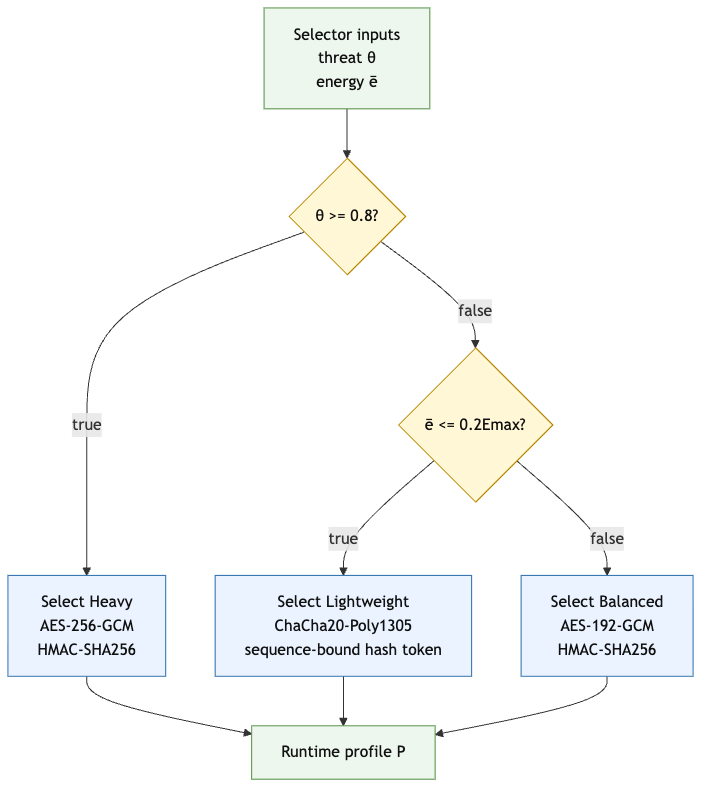
\includegraphics[width=\textwidth]{parameter_selection_flowchart.png}
\caption{Decision-tree-based algorithm for adaptive cryptographic parameter selection.}
\label{fig:parameter_selection}
\end{figure}

Figure~\ref{fig:parameter_selection} should therefore be interpreted as a simplified decision tree for the current prototype, not as a proof of global optimality.

\section{Implementation Aspects}
\label{sec:implementation_aspects}

The benchmark implementation targets a constrained but host-based execution environment. It uses Docker containers and gRPC-connected peers to emulate runtime isolation, while CPU and memory limits approximate weaker embedded hardware. The practical measurements therefore say more about software behavior under constrained execution than about the exact latency of a deployed robotic platform.

The prototype is pairwise on the measured data path. Even when a scenario file specifies more than two peers, the current benchmark focuses on the primary \texttt{peer\_a} $\rightarrow$ \texttt{peer\_b} exchange and does not claim to validate multi-hop routing, neighborhood churn, or consensus traffic. That choice keeps the benchmark reproducible and makes profile-switching behavior easy to inspect, but it also bounds the external validity of the results.

The overhead of adaptation in this prototype is negligible relative to packet protection because profile selection is a threshold check. The more meaningful costs are rekeying, data-plane protection, and queueing under CPU pressure. For that reason, the practical evaluation chapter focuses on latency, throughput, switching behavior, and a model-based energy proxy rather than on the controller itself.

Implementation guidance remains conventional. Secure random generation is required for key exchange and nonce creation; constant-time cryptographic libraries remain desirable; and any future extension toward a field-ready system would need a genuine authenticated control plane, device identity management, and deployment-specific fault handling~\cite{chenSecuringEmergentBehaviour2021}. New lightweight standards such as Ascon may also be relevant for future constrained-device variants, but they are not part of the implemented benchmark profile set~\cite{nistSP800232Ascon}.

\chapter{Practical Evaluation and Benchmark Results}
\label{chap:practical_evaluation}

\section{Retained Security Reasoning}
\label{sec:security_proofs}

Formal reasoning remains useful because the benchmark suite validates implementation behavior, not cryptographic soundness by itself. The claims retained in this thesis are intentionally narrower than full end-to-end protocol proofs.

\textbf{Confidentiality claim.}  
If the nonce discipline is respected and the underlying AEAD schemes behave as expected, then the benchmarked data plane inherits the confidentiality properties of AES-GCM and ChaCha20-Poly1305 at the profile level.

\textbf{Authentication claim.}  
If HMAC-SHA256, the implemented sequence-bound hash-token checks, and the receiver-side replay filter behave as expected, then the benchmarked data plane can reject forged runtime packets and duplicate already accepted packets within the same epoch.

These statements should not be read as full proofs of the complete adaptive architecture described earlier. In particular, the benchmark does not validate signed control-plane messages, multi-node synchronization, or broader swarm-level trust properties. The role of this section is therefore to bound the interpretation of the benchmark: the practical evaluation targets a pairwise adaptive secure-communication prototype with retained data-plane reasoning.

\section{Benchmark Implementation and Setup}
\label{sec:benchmark_setup}

The practical evaluation uses an executable benchmark suite rather than analytical performance estimates alone. The implementation instantiates two containerized peers that exchange protected messages over gRPC. Session establishment uses X25519 with HKDF-derived epoch material. Heavy and balanced modes use AES-GCM with additional HMAC-based runtime authentication, while lightweight mode uses ChaCha20-Poly1305 with a sequence-bound hash token and receiver-side duplicate rejection within each epoch. The adaptive controller switches among these profiles according to scripted threat and energy schedules.

The final benchmark pass uses the following fixed setup:
\begin{itemize}
    \item two communicating peers on the measured data path;
    \item CPU cap of 0.05 cores per peer in the main stability sweep;
    \item memory cap of 128~MiB per peer;
    \item message size of 65\,536 bytes;
    \item experiment duration of 60 seconds;
    \item three repeats per matrix cell;
    \item rekey interval of 2 seconds in the main stability sweep.
\end{itemize}

Network impairment is disabled in the main stability sweep so that the constrained CPU budget dominates the observed behavior. Threat and energy inputs are scripted rather than sensed from physical hardware. The adaptive scenario starts in a balanced low-threat regime, escalates to heavy mode at 12 seconds, returns to balanced mode at 24 seconds, switches to lightweight mode at 36 seconds under a low-energy condition, and returns to heavy mode at 48 seconds when threat rises again.

The benchmark reports the following metrics:
\begin{itemize}
    \item measured p50, p95, and p99 message latency;
    \item achieved throughput and delivered-message count;
    \item mode switches and message-profile mix for adaptive runs;
    \item drop rate against attempted sends;
    \item normalized energy proxy per delivered message;
    \item cryptographic work per delivered message, defined as bytes processed by encryption, decryption, and authentication primitives;
    \item long-run protection-tier work and policy-fit share for switching behavior;
    \item standard deviation of throughput across repeats.
\end{itemize}

The energy values reported in this chapter are \emph{model-based proxies}, not physical power measurements. They remain useful for relative comparison across profiles under the same workload, but they must not be interpreted as battery-accurate consumption.
For the figures in this chapter, the more important cost metric is cryptographic work. Unlike the energy proxy, this is not a weighted model: it is derived from raw run counters, the message-profile mix, and the bytes processed by the implemented crypto primitives.

The final artifact directory is \path{benchmarks/thesis-report-final}. It contains 228 completed benchmark summary rows from a single benchmark pass: 84 main-stability runs, 72 CPU-sensitivity runs, 36 rekey-sensitivity runs, and 36 network-impairment runs. Every matrix cell has three completed summary rows, all comparison rows contain a \texttt{source\_run\_dir}, and the generated report includes CSV, JSON, SVG, and PNG artifacts for the comparison, sweep, CPU sensitivity, rekey sensitivity, and network impairment plots.

The repository separates source artifacts from generated evidence. The benchmark package contains the executable implementation, Docker setup, scenario presets, and tests, while \path{benchmarks/thesis-report-final} contains the curated result matrix used for the tables and figures in this chapter. The public repository for the thesis artifact is available at \url{https://github.com/mazzz3r/adaptive-swarm-crypto-thesis}.

\section{Main Stability Sweep}
\label{sec:saturation_results}

The main sweep evaluates offered rates from 25 to 300 messages per second under the same 0.05-core CPU cap. Table~\ref{tab:main_stability_sweep} reports medians across three repeats per cell, with throughput standard deviation included to show run-to-run spread.

\begin{table}[H]
\centering
\scriptsize
\caption{Main stability sweep; crypto work is in MiB per delivered message}
\label{tab:main_stability_sweep}
\renewcommand{\arraystretch}{1.15}
\resizebox{\textwidth}{!}{%
\begin{tabular}{|c|l|c|c|c|c|c|c|c|c|}
\hline
\textbf{Rate} & \textbf{Mode} & \textbf{Runs} & \textbf{Med. P50} & \textbf{Med. P95} & \textbf{Med. P99} & \textbf{Med. throughput} & \textbf{Med. drop \%} & \textbf{Med. crypto work} & \textbf{Throughput std} \\
\hline
25 & Heavy & 3 & 77.606 & 294.362 & 397.421 & 25.0 & 0.000 & 0.2500 & 0.00 \\
25 & Balanced & 3 & 12.422 & 199.912 & 298.894 & 25.0 & 0.000 & 0.2500 & 0.00 \\
25 & Lightweight & 3 & 30.701 & 202.364 & 304.612 & 25.0 & 0.000 & 0.1251 & 0.01 \\
25 & Adaptive & 3 & 25.296 & 202.027 & 301.172 & 25.0 & 0.000 & 0.2248 & 0.02 \\
50 & Heavy & 3 & 197.992 & 543.232 & 795.484 & 46.3 & 6.877 & 0.2500 & 0.35 \\
50 & Balanced & 3 & 178.694 & 695.961 & 798.890 & 47.6 & 4.447 & 0.2500 & 2.00 \\
50 & Lightweight & 3 & 101.445 & 546.791 & 699.806 & 47.7 & 4.167 & 0.1251 & 0.24 \\
50 & Adaptive & 3 & 100.938 & 695.493 & 898.012 & 46.9 & 6.175 & 0.2240 & 2.30 \\
75 & Heavy & 3 & 198.307 & 697.320 & 825.192 & 56.7 & 24.356 & 0.2500 & 0.38 \\
75 & Balanced & 3 & 101.597 & 403.873 & 701.058 & 54.1 & 26.443 & 0.2500 & 6.53 \\
75 & Lightweight & 3 & 101.698 & 596.553 & 774.667 & 57.2 & 23.489 & 0.1251 & 0.58 \\
75 & Adaptive & 3 & 141.028 & 597.793 & 798.515 & 53.7 & 27.923 & 0.2257 & 2.10 \\
100 & Heavy & 3 & 124.843 & 571.559 & 825.390 & 58.4 & 40.110 & 0.2500 & 0.79 \\
100 & Balanced & 3 & 102.750 & 500.696 & 700.531 & 59.9 & 38.484 & 0.2500 & 2.67 \\
100 & Lightweight & 3 & 128.887 & 694.480 & 800.385 & 62.7 & 36.206 & 0.1251 & 2.60 \\
100 & Adaptive & 3 & 195.263 & 599.890 & 752.292 & 61.2 & 38.783 & 0.2256 & 1.56 \\
150 & Heavy & 3 & 102.715 & 695.176 & 896.869 & 67.0 & 54.025 & 0.2500 & 2.78 \\
150 & Balanced & 3 & 196.844 & 601.281 & 798.638 & 68.0 & 54.189 & 0.2500 & 4.77 \\
150 & Lightweight & 3 & 201.109 & 601.308 & 795.585 & 56.5 & 60.181 & 0.1251 & 1.42 \\
150 & Adaptive & 3 & 103.044 & 496.674 & 699.220 & 58.7 & 58.410 & 0.2221 & 4.61 \\
200 & Heavy & 3 & 200.797 & 697.407 & 901.111 & 60.9 & 68.615 & 0.2500 & 1.30 \\
200 & Balanced & 3 & 201.448 & 797.382 & 963.524 & 61.2 & 67.627 & 0.2500 & 1.34 \\
200 & Lightweight & 3 & 198.301 & 700.638 & 896.513 & 63.9 & 67.776 & 0.1251 & 2.21 \\
200 & Adaptive & 3 & 199.721 & 699.131 & 902.077 & 59.6 & 69.764 & 0.2243 & 1.01 \\
300 & Heavy & 3 & 198.630 & 699.370 & 898.656 & 62.0 & 77.631 & 0.2500 & 1.10 \\
300 & Balanced & 3 & 200.033 & 695.980 & 895.410 & 63.1 & 78.873 & 0.2500 & 0.86 \\
300 & Lightweight & 3 & 198.126 & 795.373 & 901.518 & 61.0 & 75.341 & 0.1251 & 1.90 \\
300 & Adaptive & 3 & 199.256 & 697.619 & 899.595 & 63.7 & 78.447 & 0.2230 & 2.58 \\
\hline
\end{tabular}
}
\end{table}

\begin{figure}[H]
\centering
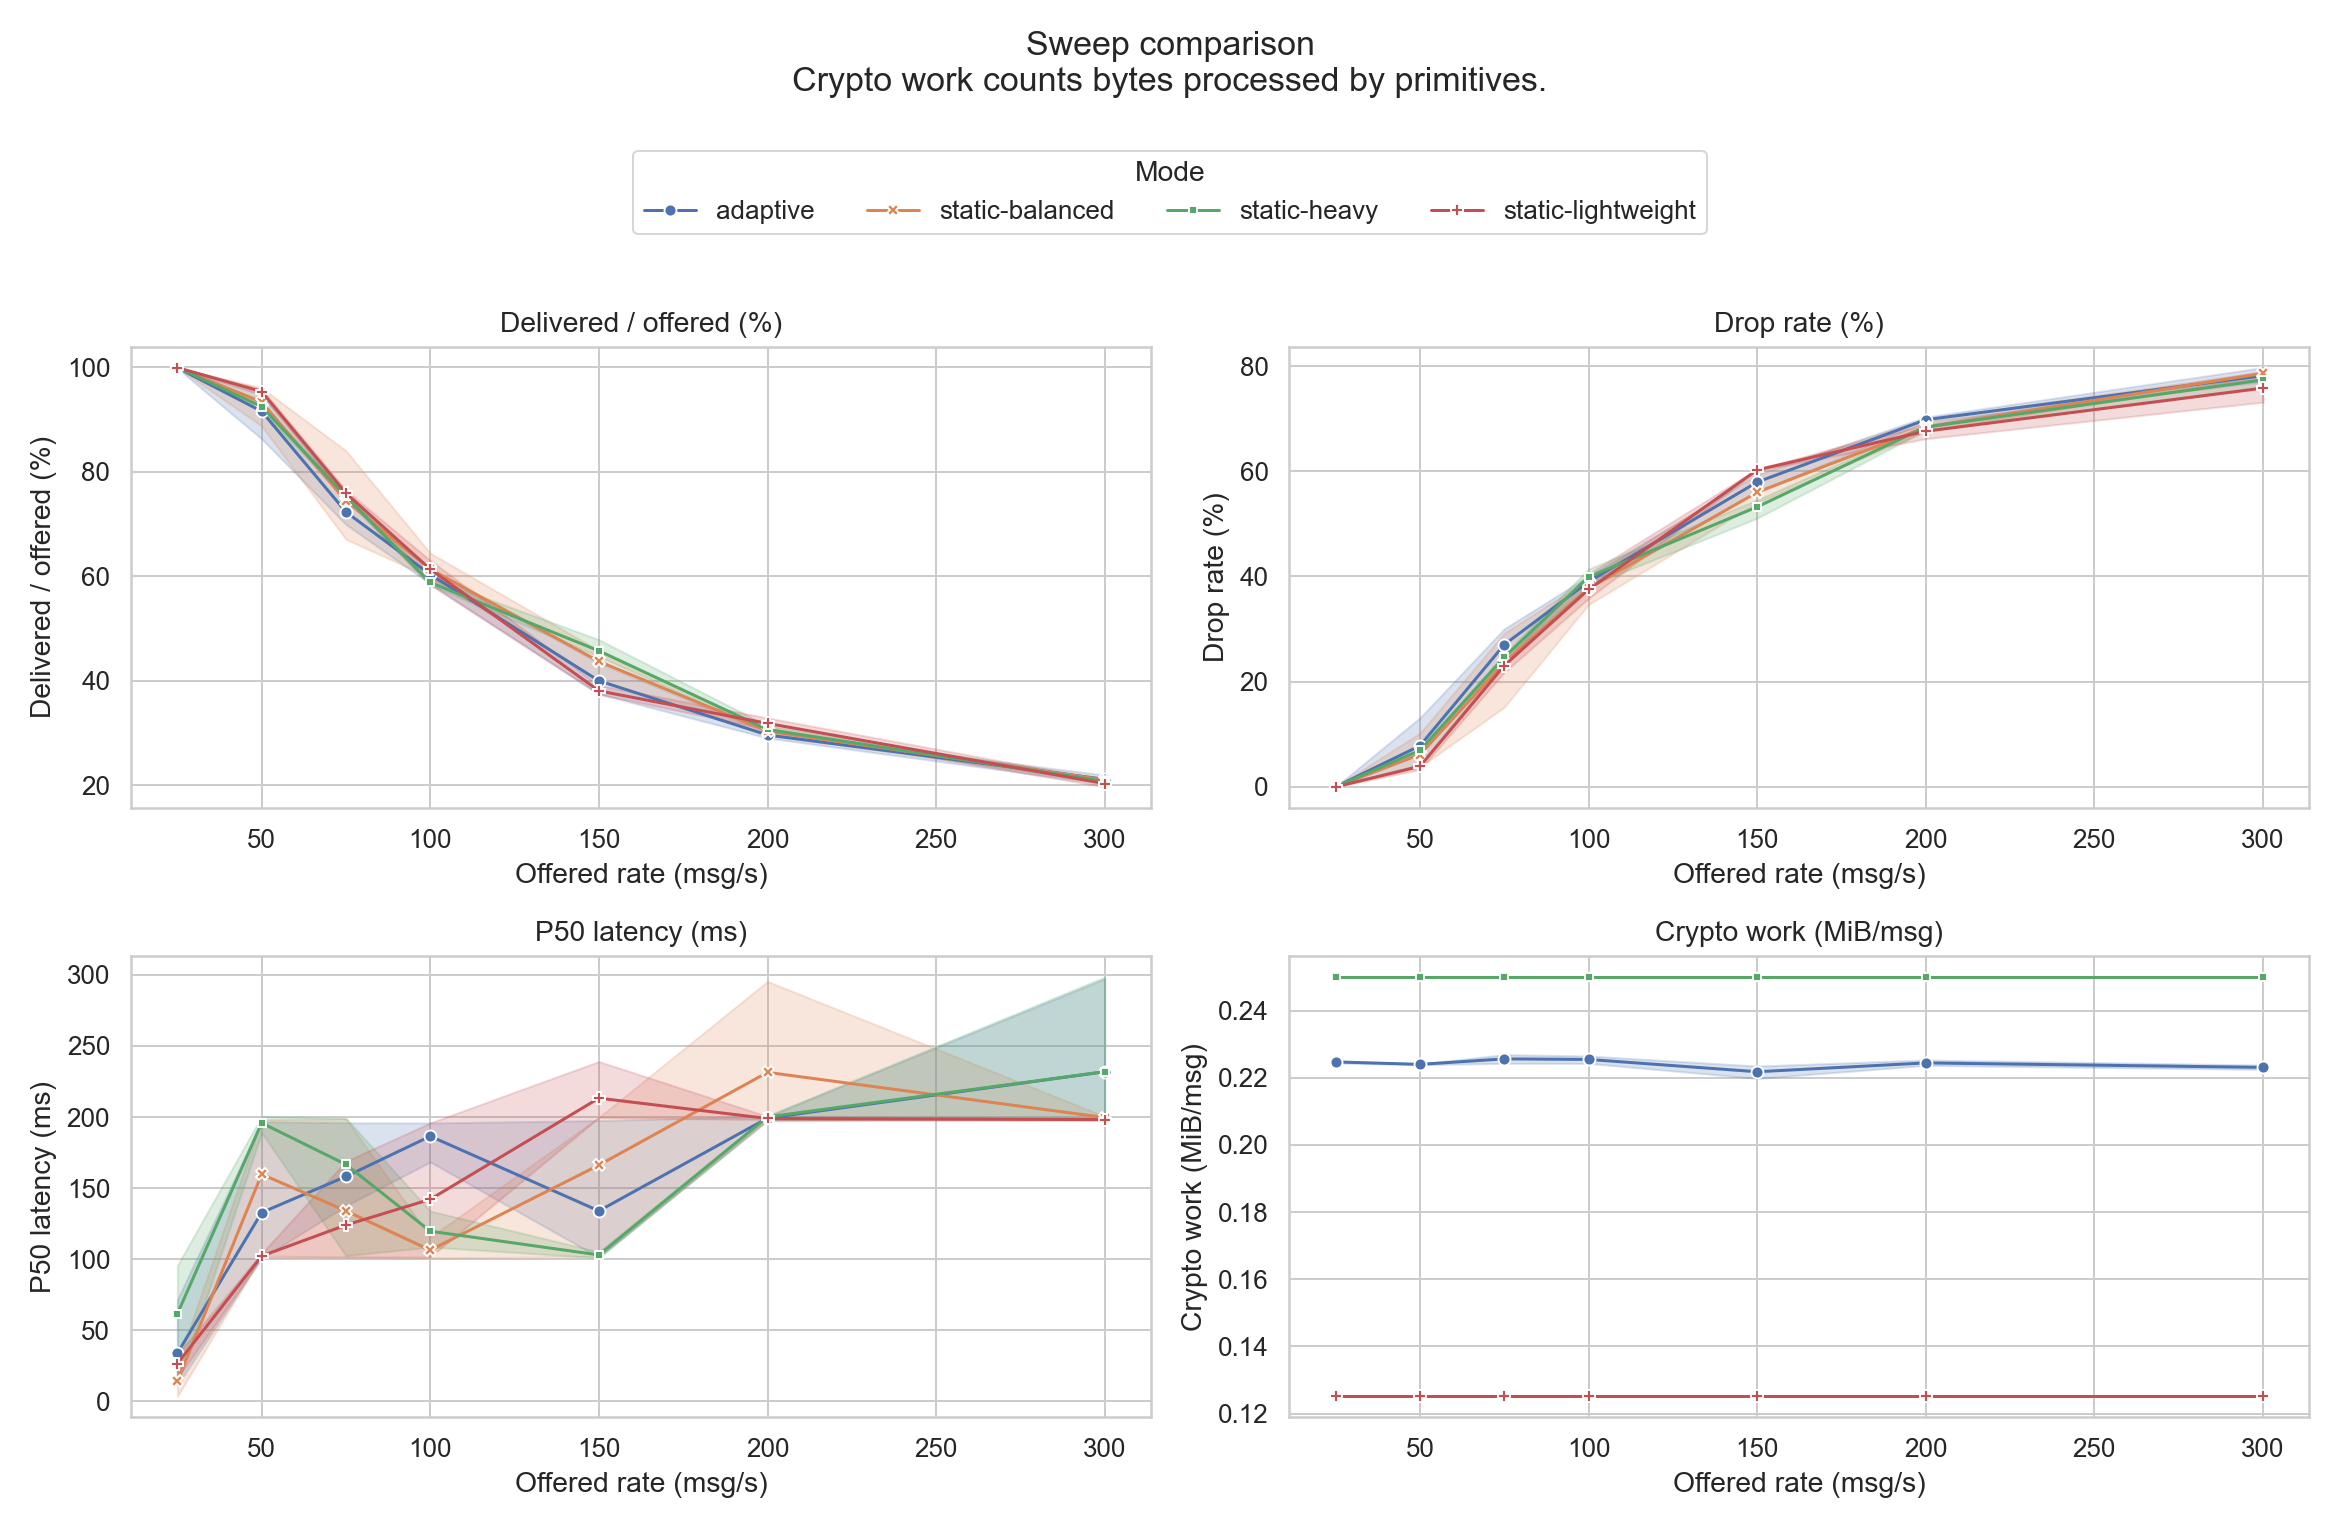
\includegraphics[width=\textwidth]{figs/benchmark_sweep_metrics.png}
\caption{Main stability sweep metrics: delivery ratio, drop rate, latency, and cryptographic work per delivered message.}
\label{fig:benchmark_sweep_metrics}
\end{figure}

The sweep shows a clear knee between 25 and 75 messages per second under the 0.05-core cap on the host system. At 25 messages per second all four strategies deliver the full offered rate. At 50 messages per second the prototype already starts dropping a small share of messages, and by 75--100 messages per second it is CPU- and queue-limited. Above that point, increasing the offered rate mostly increases sender-side drops rather than delivered throughput. Figure~\ref{fig:benchmark_sweep_metrics} makes this saturation effect explicit by plotting delivered throughput as a fraction of offered load.

The close spacing of the delivery, drop-rate, and latency curves is expected for this long-run end-to-end setup. These panels measure the whole containerized gRPC pipeline, so shared queueing, scheduling, serialization, and payload-transfer costs dominate once the run is near saturation. The profile-specific difference is therefore shown separately as cryptographic work. Heavy and balanced modes process about twice as many crypto primitive bytes per delivered message as lightweight mode because they add an HMAC authentication pass on top of AEAD encryption and decryption. Adaptive remains between the authenticated static profiles and lightweight mode because it spends only part of the run in lightweight mode.

\begin{figure}[H]
\centering
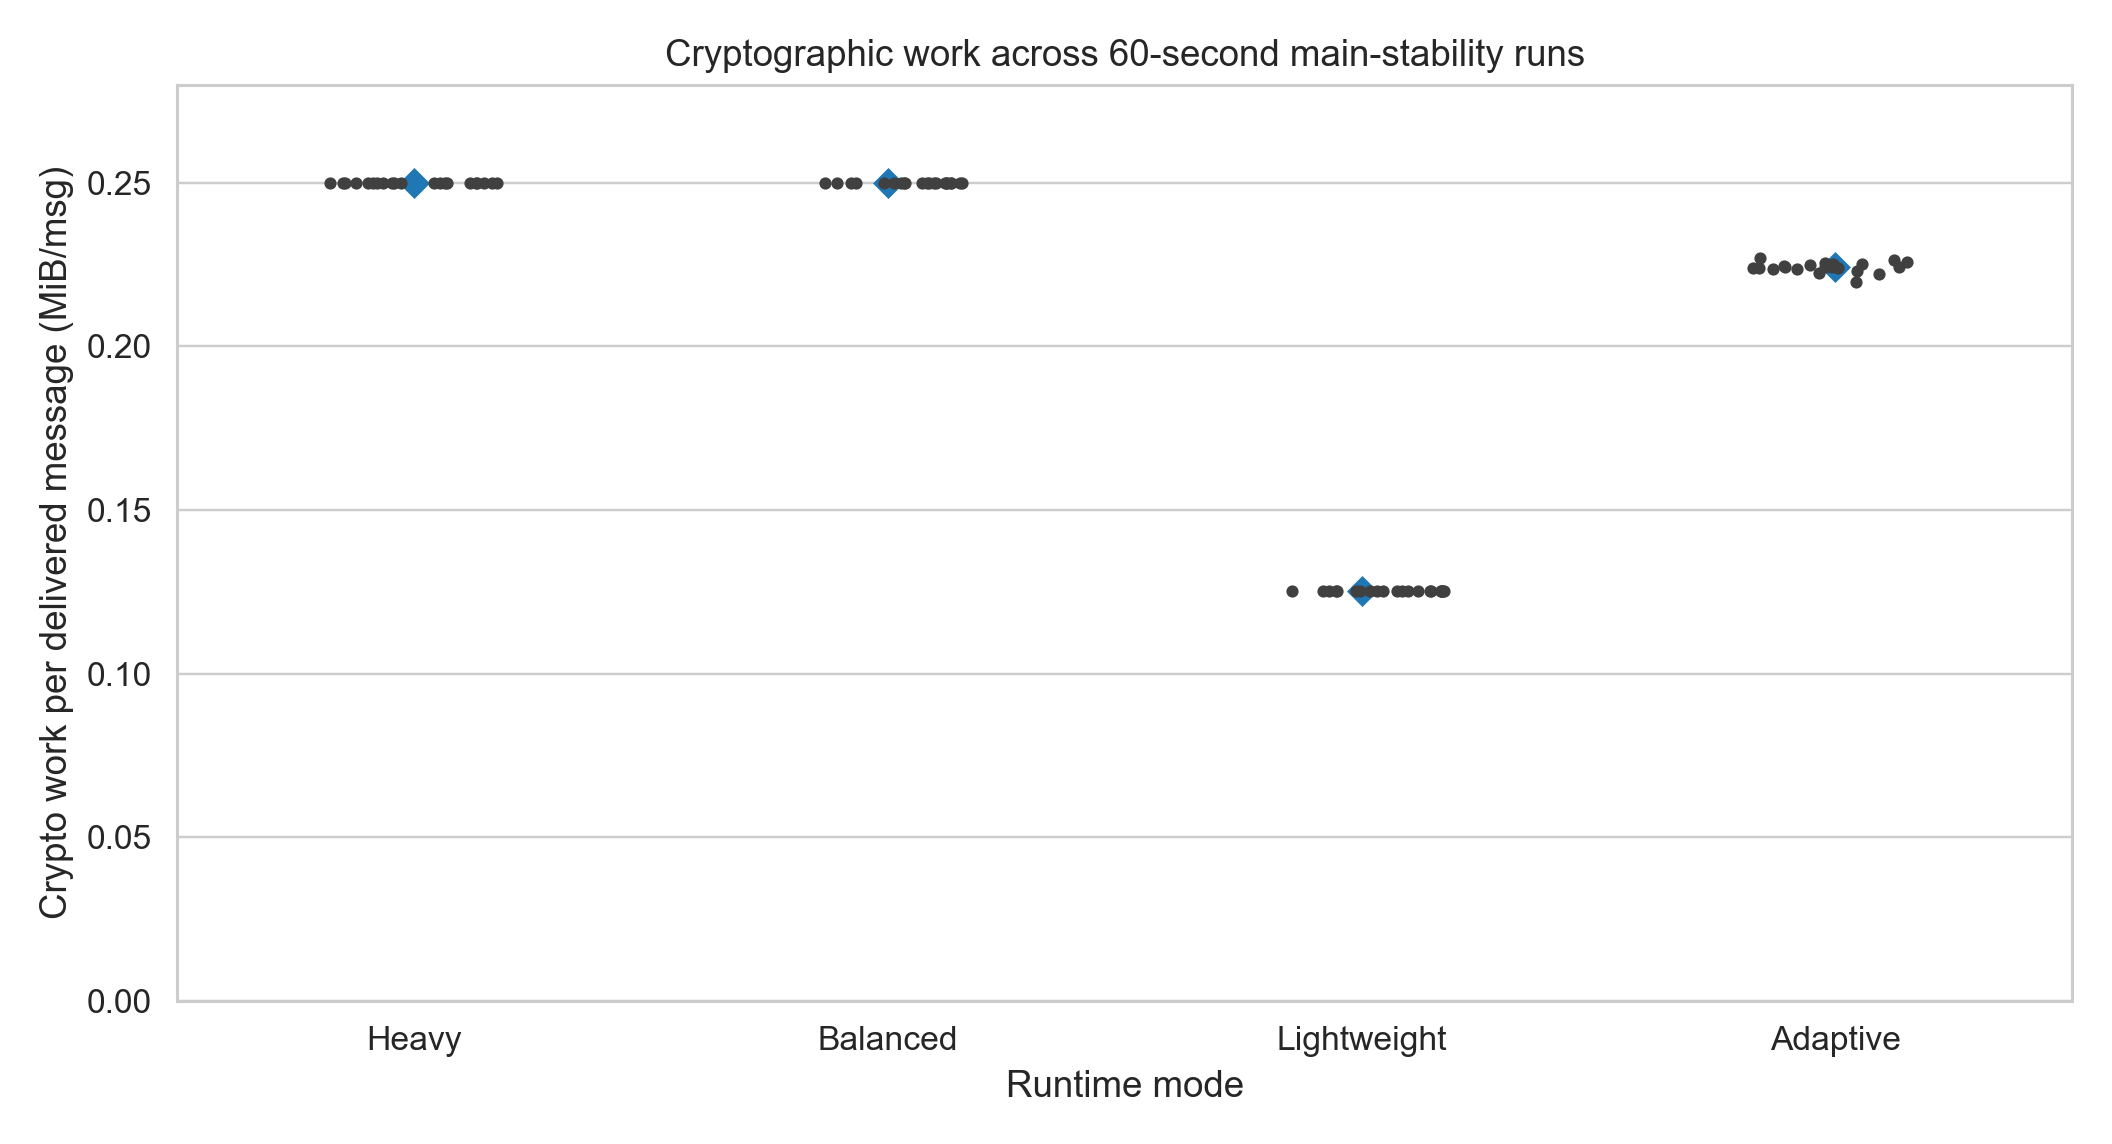
\includegraphics[width=0.86\textwidth]{figs/benchmark_crypto_work_profile.png}
\caption{Long-run cryptographic work across all 60-second main-stability runs; black points are individual runs and blue diamonds are medians.}
\label{fig:benchmark_crypto_work_profile}
\end{figure}

Across the main-stability runs, the median cryptographic work per delivered message is 0.250~MiB for heavy mode, 0.250~MiB for balanced mode, 0.224~MiB for adaptive mode, and 0.125~MiB for lightweight mode. Balanced is not identical to heavy: it uses AES-192-GCM rather than AES-256-GCM. However, the deterministic crypto-work metric counts bytes processed by primitives, not AES round count or key length. Since both heavy and balanced perform one AEAD pass plus one HMAC pass over the same delivered payload, they appear equal in byte-level crypto work. Figure~\ref{fig:benchmark_crypto_work_profile} is therefore the clearest long-run view of primitive-byte workload, while Figure~\ref{fig:benchmark_long_run_policy_tradeoff} shows the ordinal protection-level trade-off. Adaptive is not universally best; it reacts correctly to policy inputs and trades some efficiency for stronger protection during high-threat phases.

Figure~\ref{fig:benchmark_long_run_policy_tradeoff} makes the switching benefit more explicit. It compares four strategies against the same 60-second threat and energy schedule: always-heavy, always-balanced, always-lightweight, and adaptive switching. The middle panel uses protection-tier work rather than wall-clock latency: lightweight contributes one tier-message unit per message, balanced contributes two, and heavy contributes three. This metric is not an energy model; it is an ordinal policy-cost view used to show whether a strategy spends protection budget in the right part of the run.

\begin{figure}[H]
\centering
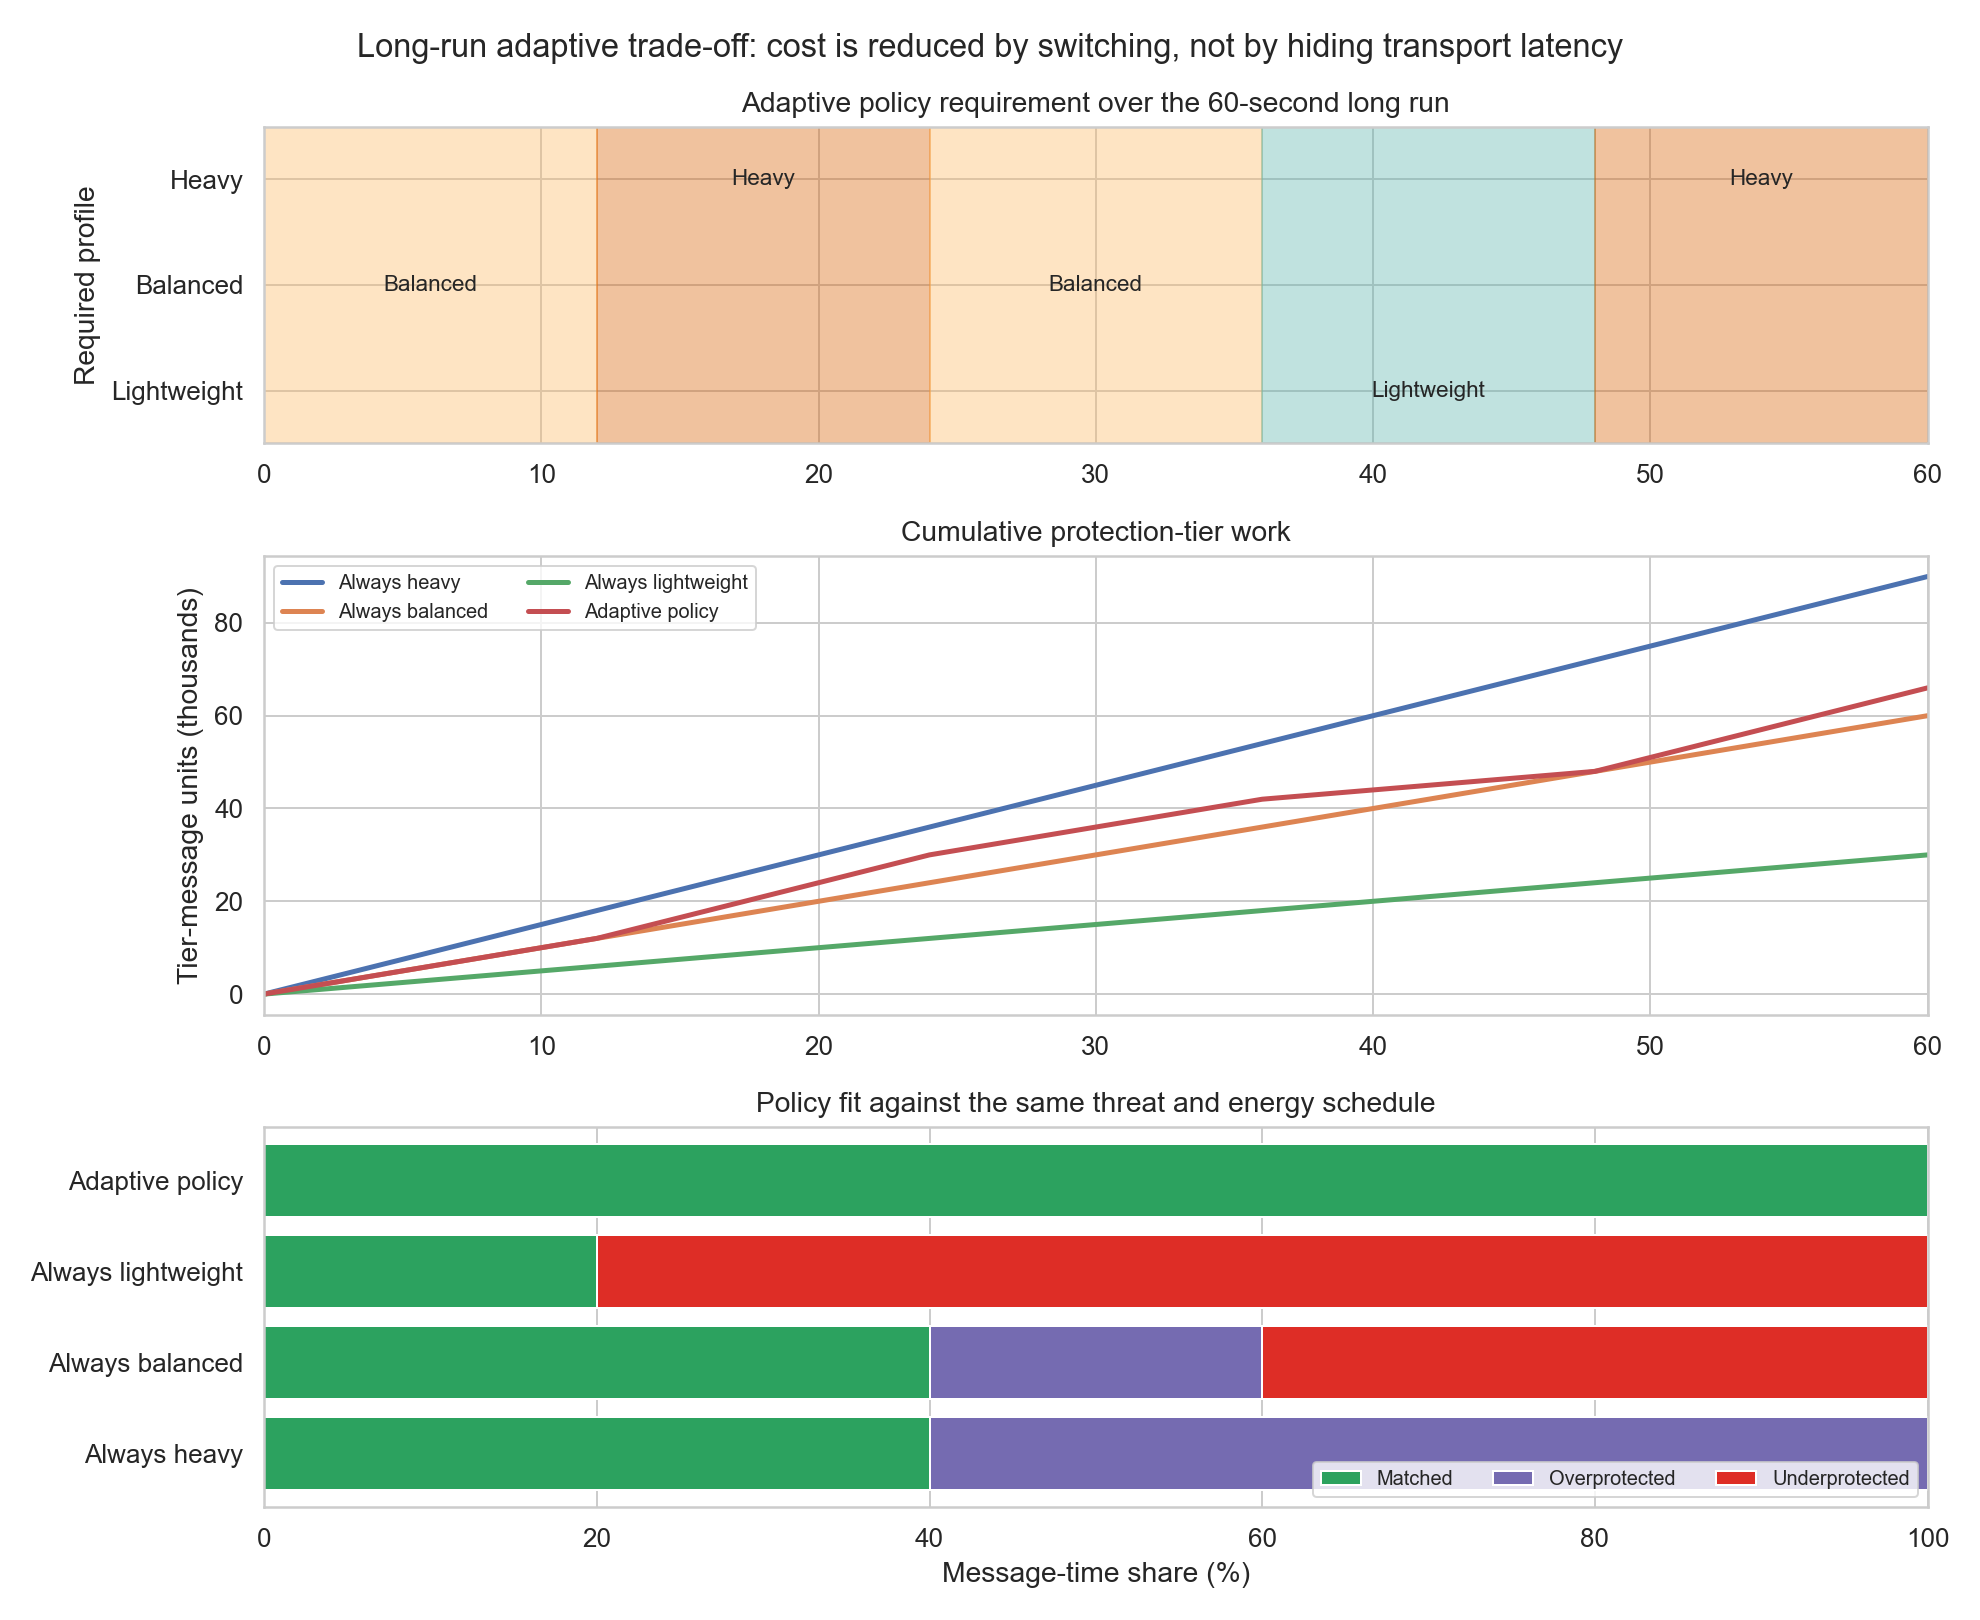
\includegraphics[width=\textwidth]{figs/benchmark_long_run_policy_tradeoff.png}
\caption{Long-run policy trade-off under the scripted threat and energy schedule.}
\label{fig:benchmark_long_run_policy_tradeoff}
\end{figure}

The always-heavy baseline reaches 90 thousand tier-message units and never underprotects, but it overprotects 60\% of the message-time. The always-lightweight baseline uses only 30 thousand tier-message units, but it underprotects 80\% of the message-time. The always-balanced baseline is the static middle point at 60 thousand tier-message units: it matches the balanced portions of the run, but it still underprotects the high-threat windows and overprotects the low-energy window. Adaptive switching reaches 66 thousand tier-message units, saves 26.7\% relative to always-heavy, and matches the required profile for the full schedule. This is the concrete advantage of the balanced/adaptive policy: it is not a large end-to-end latency gap on the host system, but a correct allocation of protection level over time.

\section{Adaptive Switching Behavior}
\label{sec:adaptive_switching}

Adaptive behavior is evaluated both through aggregate metrics and through the recorded switching trace. A representative clean 100~Hz main-stability run recorded four transitions: heavy mode at 12.062 seconds because of high threat, balanced mode at 24.065 seconds when threat fell, lightweight mode at 36.162 seconds under the low-energy condition, and heavy mode again at 48.067 seconds when threat rose. The same run sent 1\,486 heavy-profile messages, 1\,432 balanced-profile messages, and 755 lightweight-profile messages.

Across all 57 adaptive runs, 54 recorded the expected four transitions. The three exceptions are all in the deliberately severe lossy-network profile: two runs recorded zero transitions and one recorded only one transition because the run effectively collapsed under impairment, with sender-side drop rates between 75.566\% and 94.312\%. This is not evidence that the adaptive policy failed under normal conditions; it is evidence that the current containerized transport can become too impaired for the scripted policy timeline to be fully exercised.

\begin{figure}[H]
\centering
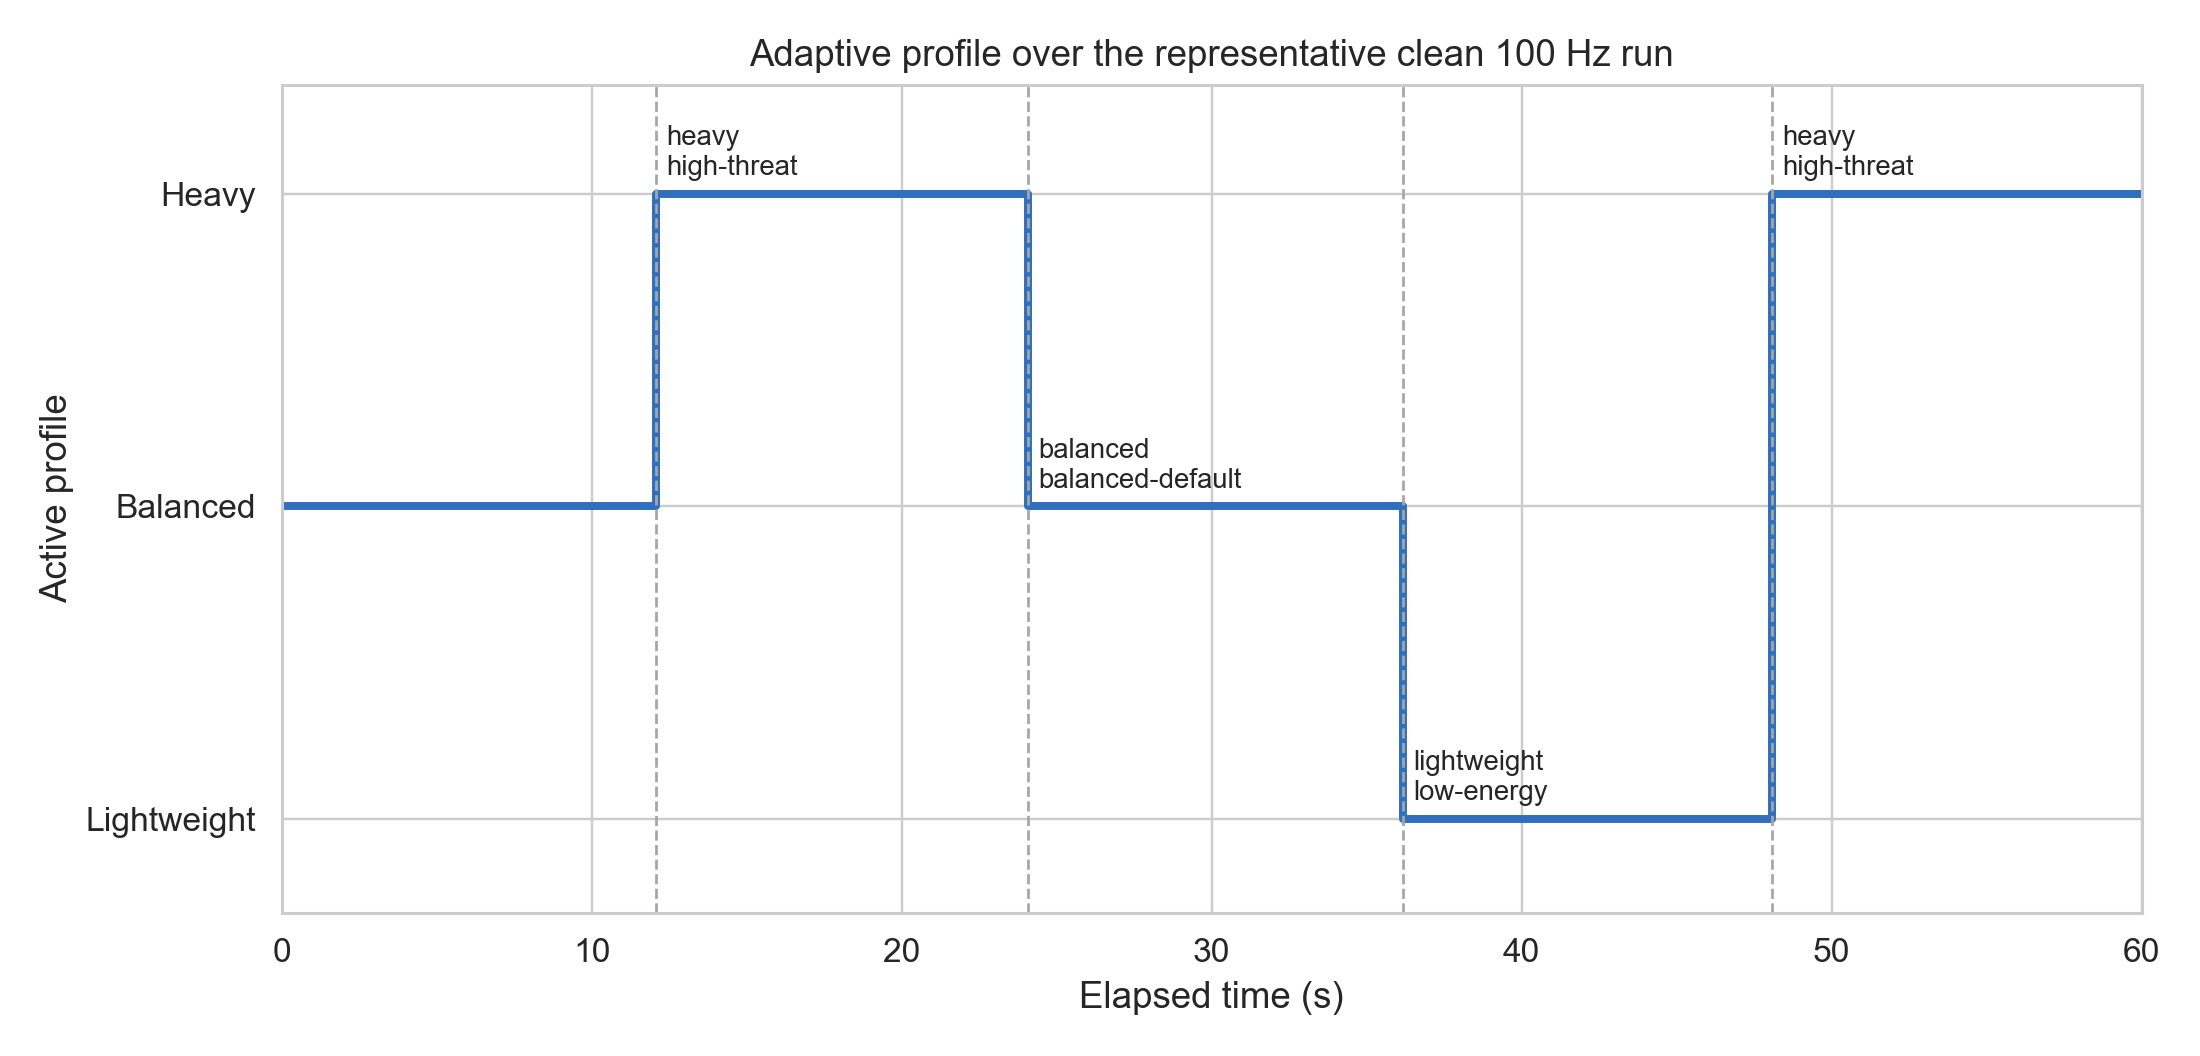
\includegraphics[width=\textwidth]{figs/benchmark_adaptive_switches.png}
\caption{Adaptive switching trace for the representative clean 100~Hz main-stability run.}
\label{fig:benchmark_adaptive_switches}
\end{figure}

\section{Sensitivity Analysis}
\label{sec:sensitivity_analysis}

The final evidence pass includes three targeted sensitivity checks: CPU cap, rekey interval, and network impairment. Table~\ref{tab:cpu_sensitivity} reports the stressed 200~Hz CPU-sensitivity subset. The 100~Hz CPU-sensitivity runs show the same qualitative behavior: CPU caps of 0.10 and 0.25 cores remove the drop observed at 0.05 cores.

\begin{table}[H]
\centering
\small
\caption{CPU sensitivity at 200~Hz; crypto work is in MiB per delivered message}
\label{tab:cpu_sensitivity}
\renewcommand{\arraystretch}{1.15}
\resizebox{\textwidth}{!}{%
\begin{tabular}{|c|l|c|c|c|c|}
\hline
\textbf{CPU cap} & \textbf{Mode} & \textbf{Med. P50} & \textbf{Med. throughput} & \textbf{Med. drop \%} & \textbf{Med. crypto work} \\
\hline
0.05 & Heavy & 198.387 & 60.5 & 68.860 & 0.2500 \\
0.05 & Balanced & 103.972 & 65.7 & 66.832 & 0.2500 \\
0.05 & Lightweight & 194.513 & 69.8 & 64.612 & 0.1251 \\
0.05 & Adaptive & 195.289 & 76.4 & 61.585 & 0.2265 \\
0.10 & Heavy & 97.266 & 147.7 & 26.002 & 0.2500 \\
0.10 & Balanced & 96.721 & 151.9 & 23.930 & 0.2500 \\
0.10 & Lightweight & 97.791 & 151.2 & 24.204 & 0.1251 \\
0.10 & Adaptive & 96.506 & 155.4 & 21.873 & 0.2252 \\
0.25 & Heavy & 1.062 & 200.0 & 0.000 & 0.2500 \\
0.25 & Balanced & 1.156 & 200.0 & 0.000 & 0.2500 \\
0.25 & Lightweight & 1.138 & 200.0 & 0.000 & 0.1251 \\
0.25 & Adaptive & 1.093 & 200.0 & 0.000 & 0.2250 \\
\hline
\end{tabular}
}
\end{table}

\begin{figure}[H]
\centering
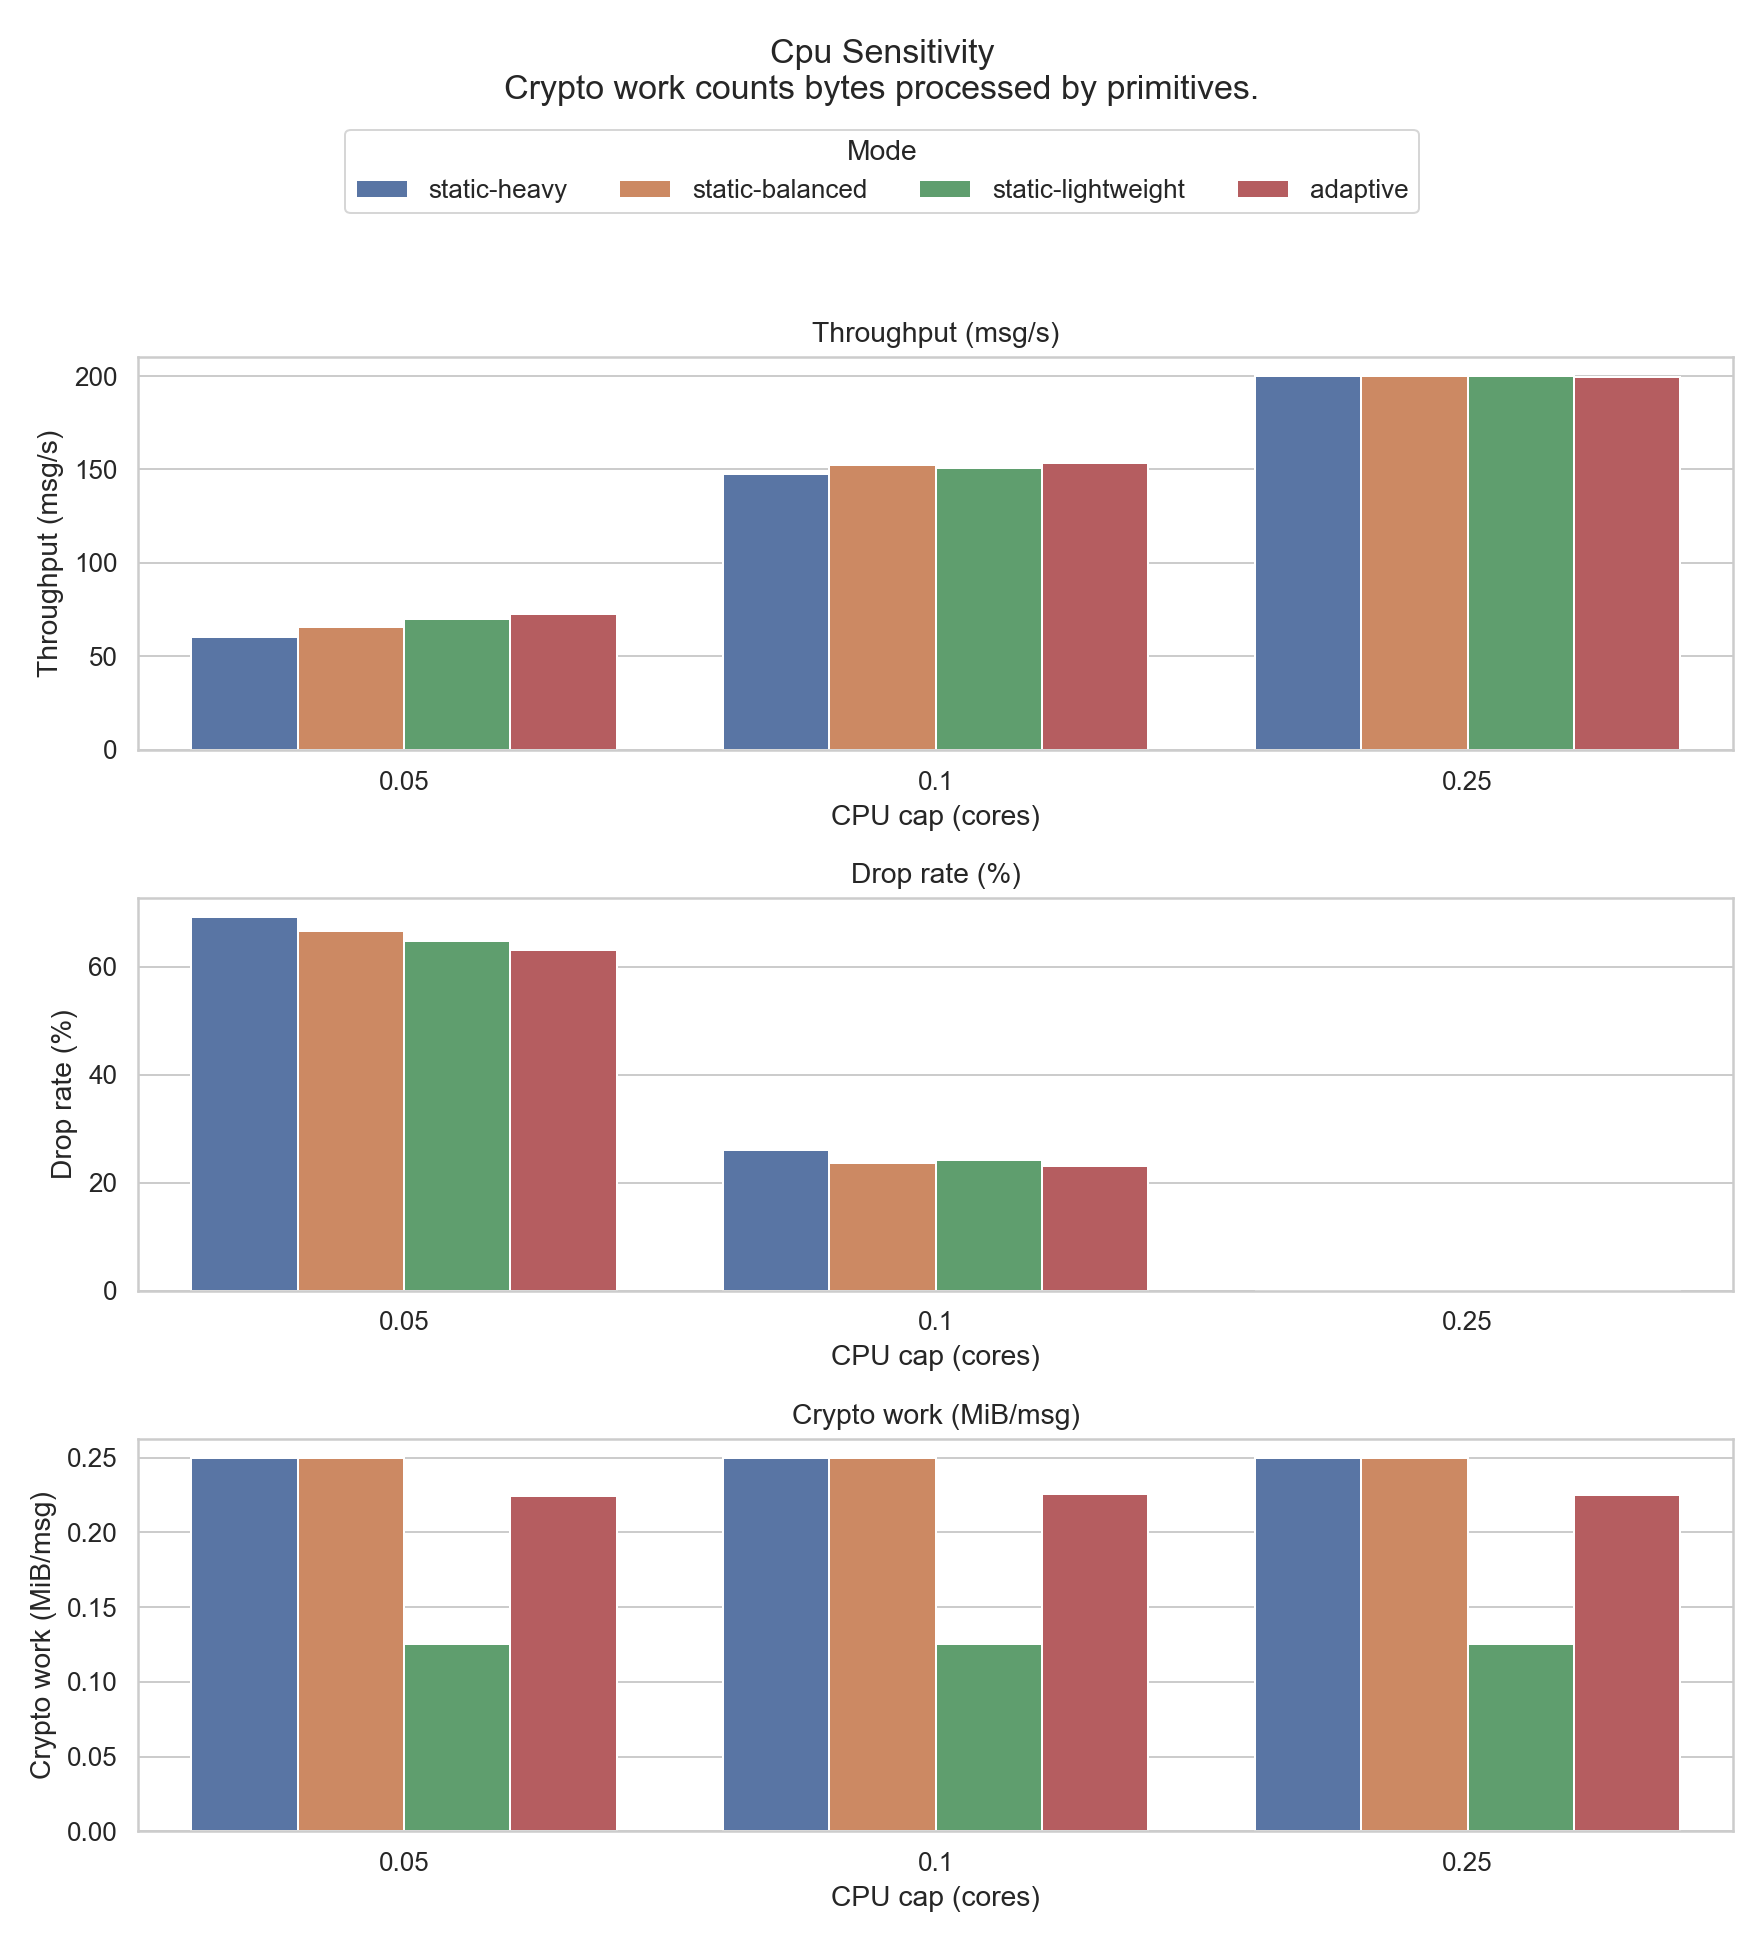
\includegraphics[width=\textwidth]{figs/benchmark_cpu_sensitivity.png}
\caption{CPU sensitivity at 200~Hz: throughput, drop rate, and cryptographic work.}
\label{fig:benchmark_cpu_sensitivity}
\end{figure}

The CPU sensitivity result is the strongest explanation for the saturation behavior. Under the 0.05-core cap, the prototype cannot sustain 200 messages per second and drops roughly 62--69\% of attempted sends. At 0.10 cores the same workload improves substantially but still drops about 22--26\%, while at 0.25 cores it is sustained cleanly in all four modes. This supports the conclusion that the main sweep is CPU-limited rather than limited by the nominal cryptographic design alone. The cryptographic-work panel remains separated because it counts profile-specific primitive work rather than shared end-to-end queueing delay.

Table~\ref{tab:rekey_sensitivity} shows the rekey-interval sensitivity at 100~Hz. In this benchmark pass, changing the rekey interval does not dominate the result: all rows remain close to the same queueing boundary under the 0.05-core cap. This makes the rekey experiment a stability check rather than evidence that a longer interval alone solves the throughput bottleneck.

\begin{table}[H]
\centering
\small
\caption{Rekey sensitivity at 100~Hz and 0.05 CPU cores; crypto work is in MiB per delivered message}
\label{tab:rekey_sensitivity}
\renewcommand{\arraystretch}{1.15}
\resizebox{\textwidth}{!}{%
\begin{tabular}{|c|l|c|c|c|c|}
\hline
\textbf{Rekey interval} & \textbf{Mode} & \textbf{Med. P50} & \textbf{Med. throughput} & \textbf{Med. drop \%} & \textbf{Med. crypto work} \\
\hline
2s & Heavy & 200.406 & 60.0 & 39.325 & 0.2500 \\
2s & Balanced & 201.038 & 63.0 & 36.983 & 0.2500 \\
2s & Lightweight & 199.882 & 62.2 & 37.833 & 0.1251 \\
2s & Adaptive & 201.078 & 60.8 & 38.151 & 0.2239 \\
5s & Heavy & 120.811 & 62.6 & 36.731 & 0.2500 \\
5s & Balanced & 201.605 & 55.5 & 44.167 & 0.2500 \\
5s & Lightweight & 265.201 & 55.4 & 42.768 & 0.1251 \\
5s & Adaptive & 200.346 & 56.1 & 42.277 & 0.2237 \\
10s & Heavy & 293.734 & 54.4 & 43.858 & 0.2500 \\
10s & Balanced & 204.749 & 54.9 & 44.334 & 0.2500 \\
10s & Lightweight & 199.739 & 55.4 & 43.357 & 0.1251 \\
10s & Adaptive & 201.683 & 55.9 & 43.604 & 0.2237 \\
\hline
\end{tabular}
}
\end{table}

\begin{figure}[H]
\centering
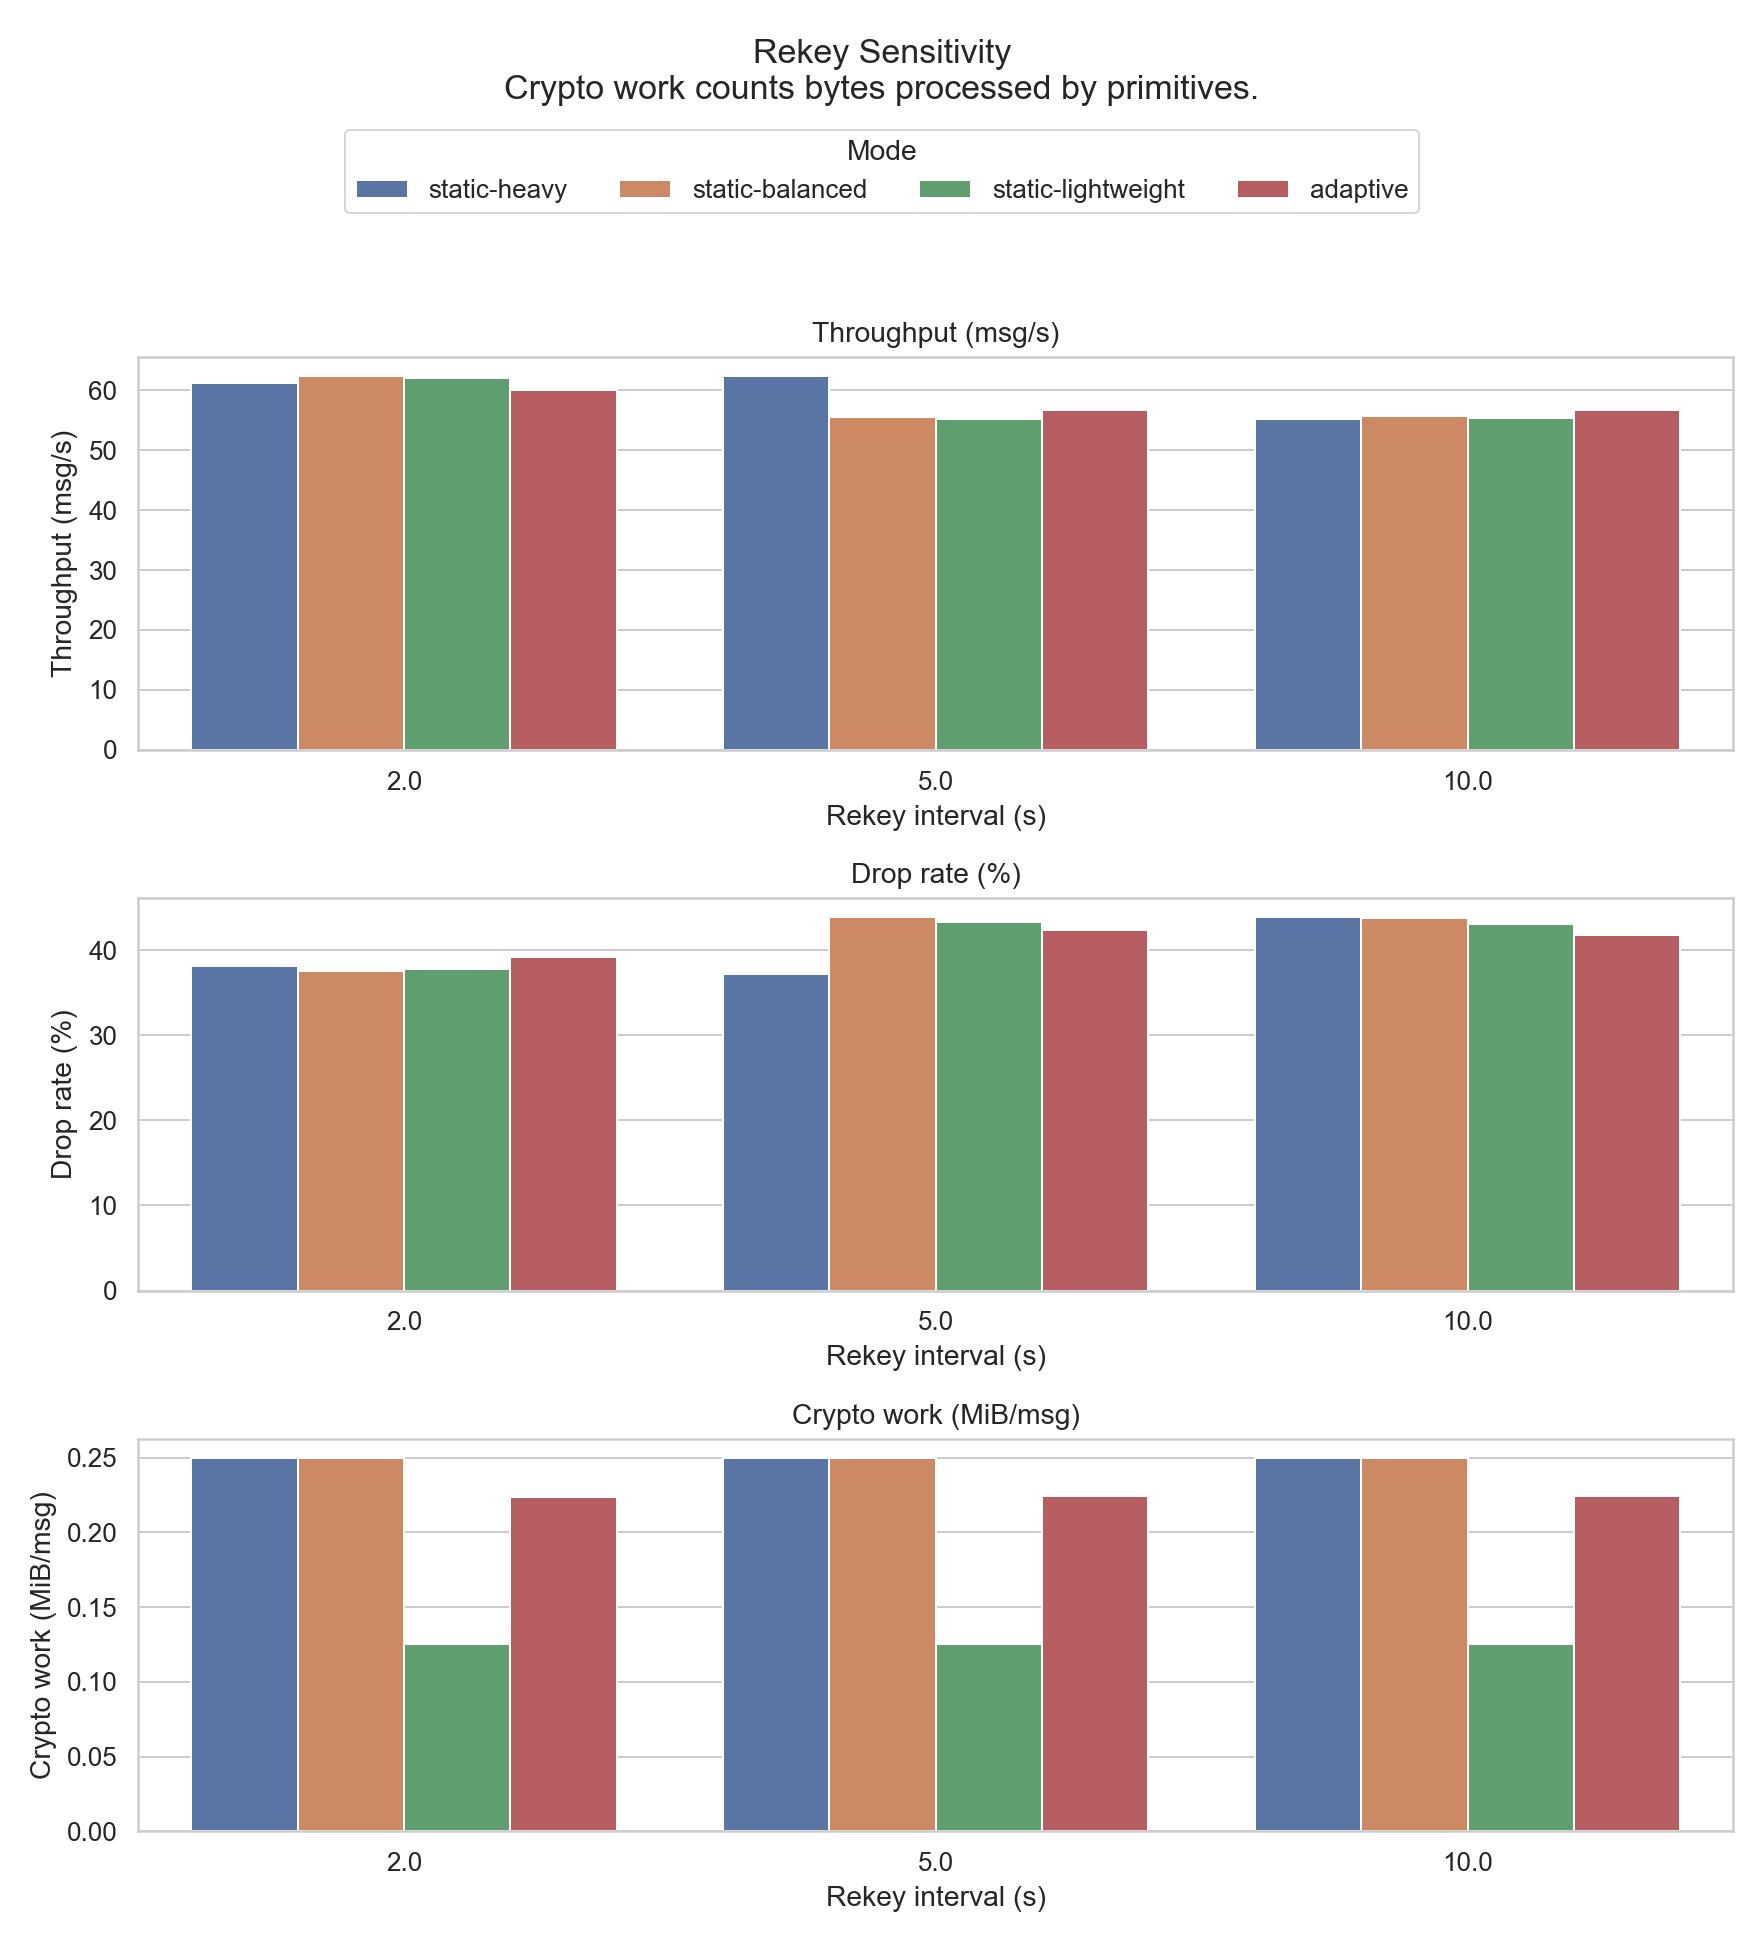
\includegraphics[width=\textwidth]{figs/benchmark_rekey_sensitivity.png}
\caption{Rekey-interval sensitivity at 100~Hz and 0.05 CPU cores, including cryptographic work.}
\label{fig:benchmark_rekey_sensitivity}
\end{figure}

Table~\ref{tab:network_impairment} reports the network-impairment sweep. The clean profile is consistent with the main 100~Hz result. The mild and lossy profiles sharply reduce delivered throughput and increase drop rate, which shows that the benchmark can expose transport-level fragility rather than hiding it behind crypto-only measurements. The impairment profiles jointly vary delay, jitter, and packet loss: clean uses 0/0/0, mild uses 20/5/2, and lossy uses 50/15/5. Figure~\ref{fig:benchmark_network_impairment} uses grouped bars rather than overlaid lines because the intended reading is the network-level collapse from clean to impaired conditions, not a fine-grained profile ordering inside each impaired condition. All 36 network-impairment runs completed, but the lossy rows should still be interpreted as transport collapse under deliberately severe delay, jitter, and packet-loss settings, not as stable steady-state performance of the cryptographic profiles. In these impaired runs, the reported drop rate includes both backlog-induced unsent attempts and explicit send errors observed by the sender.

\begin{table}[H]
\centering
\small
\caption{Network impairment at 100~Hz; crypto work is in MiB per delivered message}
\label{tab:network_impairment}
\renewcommand{\arraystretch}{1.15}
\resizebox{\textwidth}{!}{%
\begin{tabular}{|l|l|c|c|c|c|}
\hline
\textbf{Network} & \textbf{Mode} & \textbf{Med. P50} & \textbf{Med. throughput} & \textbf{Med. drop \%} & \textbf{Med. crypto work} \\
\hline
Clean & Heavy & 199.173 & 56.5 & 42.650 & 0.2500 \\
Clean & Balanced & 200.178 & 52.2 & 47.581 & 0.2500 \\
Clean & Lightweight & 201.536 & 50.9 & 48.637 & 0.1251 \\
Clean & Adaptive & 200.773 & 54.6 & 44.068 & 0.2239 \\
Mild & Heavy & 1575.028 & 11.9 & 87.907 & 0.2500 \\
Mild & Balanced & 1705.948 & 10.6 & 88.523 & 0.2500 \\
Mild & Lightweight & 1195.236 & 13.9 & 85.990 & 0.1251 \\
Mild & Adaptive & 1641.189 & 10.2 & 89.793 & 0.2243 \\
Lossy & Heavy & 2387.132 & 1.1 & 96.924 & 0.2267 \\
Lossy & Balanced & 2034.417 & 0.5 & 99.470 & 0.2348 \\
Lossy & Lightweight & 1000.831 & 1.6 & 84.953 & 0.1180 \\
Lossy & Adaptive & 1045.680 & 1.8 & 85.128 & 0.2126 \\
\hline
\end{tabular}
}
\end{table}

\begin{figure}[H]
\centering
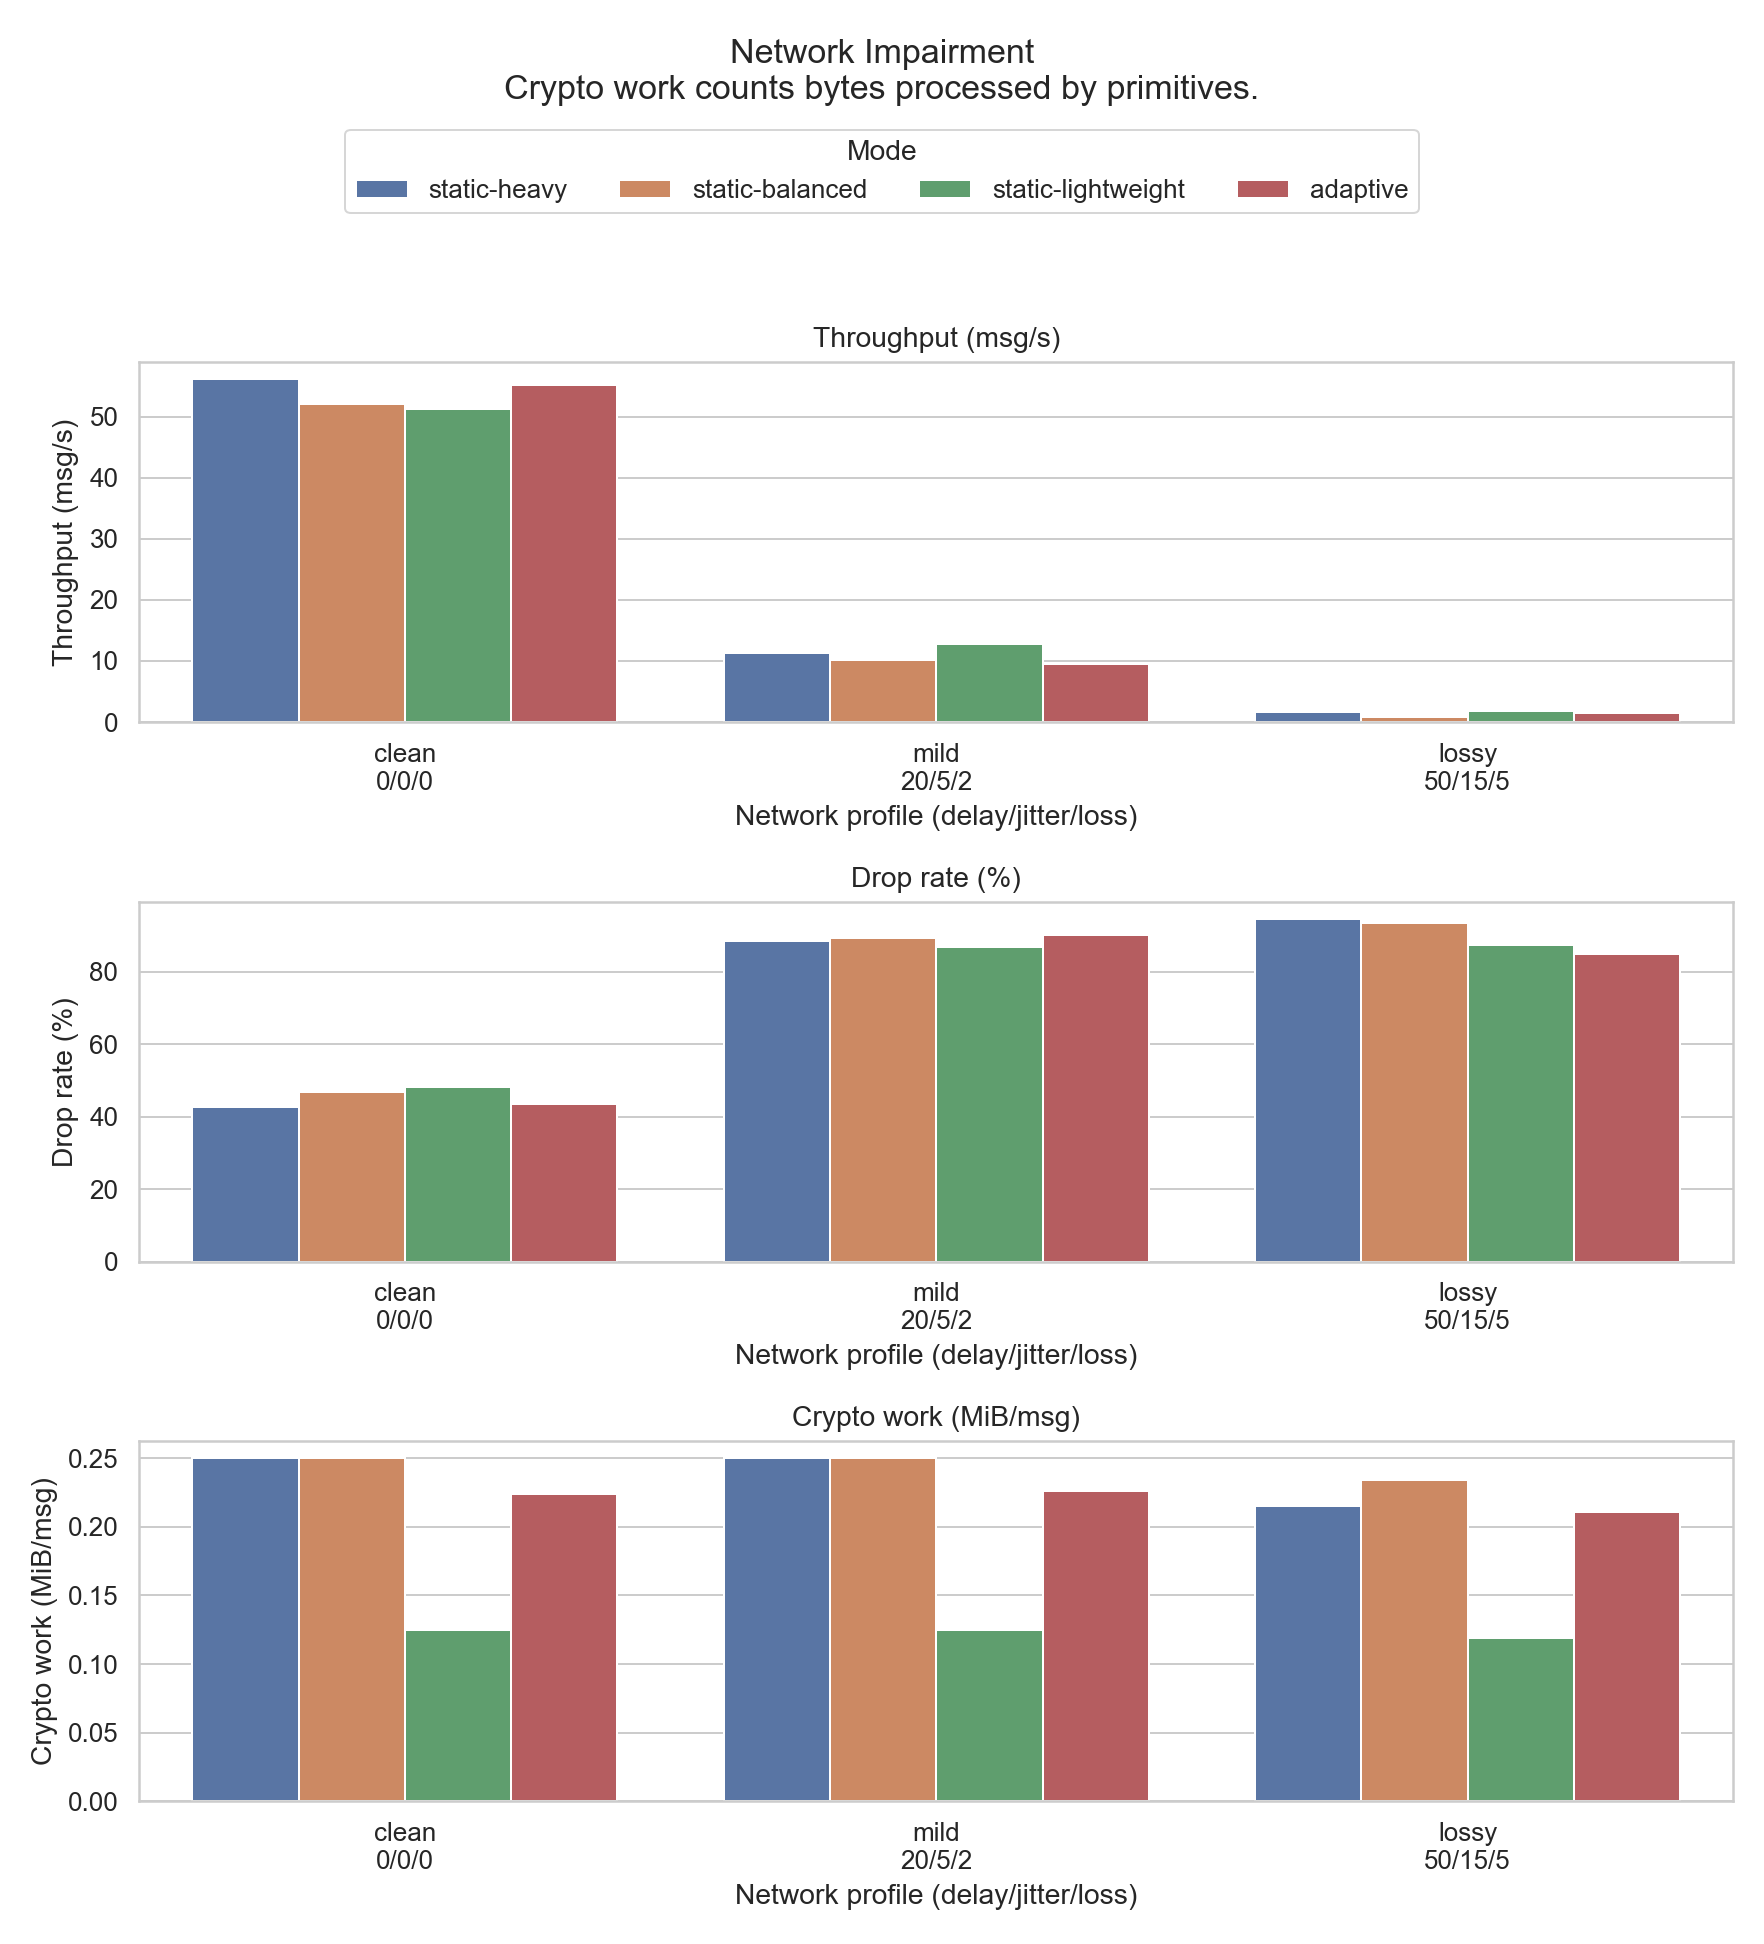
\includegraphics[width=\textwidth]{figs/benchmark_network_impairment.png}
\caption{Network-impairment sensitivity at 100~Hz; profile labels are delay/jitter/loss.}
\label{fig:benchmark_network_impairment}
\end{figure}

\section{Practical Findings}
\label{sec:practical_findings}

The final benchmark results support five practical conclusions.
\begin{itemize}
    \item Lightweight mode is the strongest default among the tested profiles when compute is the dominant constraint and maximum protection is not required at every instant: it has the lowest cryptographic work per delivered message and generally the highest sustained throughput in the repeated main sweep.
    \item Adaptive mode behaves correctly as a policy-driven compromise: it reacts to scripted runtime conditions and trades efficiency for stronger protection during high-threat periods. It should not be described as universally best.
    \item Heavy and balanced modes remain relevant authenticated operating points, but their HMAC authentication pass shows up as consistently higher cryptographic work per delivered message than lightweight mode.
    \item Offered-load experiments must be interpreted through attempted rate, delivered throughput, and drop rate together. Under the strict CPU cap, higher nominal offered rates mostly increase backlog and drops rather than proving linear scaling.
    \item Close end-to-end curves are not evidence that the benchmark is uninformative. They show that, for this containerized long-run setup and 65\,536-byte messages, transport and CPU scheduling dominate measured latency once the system is near saturation.
\end{itemize}

These findings are stronger than purely analytical estimates because they are tied to executable artifacts and repeated runs. They remain narrower than a field study. The practical evaluation validates a constrained pairwise prototype running in containers, not a complete multi-hop or large-swarm secure-communication stack, and the energy metric remains a model-based proxy rather than a physical power measurement. The cryptographic-work metric is not a power measurement either, but it is derived from raw execution counters rather than chosen energy coefficients.

\chapter{Discussion and Applications}
\label{chap:discussion}

\section{Design Guidelines}
\label{sec:design_guidelines}

The benchmarked prototype supports a limited but still useful set of design guidelines. They should be read as deployment-oriented heuristics derived from the architecture and from the pairwise benchmark evidence, not as fully field-validated prescriptions.

\textbf{Scenario 1: Disaster Response.}  
When communication reliability and energy preservation matter simultaneously, the benchmark results suggest starting from a balanced or lightweight default and reserving the heavy profile for explicitly elevated threat periods.

\textbf{Scenario 2: Agricultural Robotics.}  
Long-duration sensing missions favor lighter defaults. In the current profile set, lightweight operation minimizes the normalized energy proxy per delivered message under constrained compute and also delivers the highest measured throughput in the benchmarked sweep.

\textbf{Scenario 3: Underwater or Low-Bandwidth Links.}  
When software efficiency matters more than hardware AES acceleration, the lightweight profile remains attractive because it minimizes normalized per-message cost in the measured prototype. This is an extrapolation from the benchmark, not a dedicated underwater experiment.

\textbf{Scenario 4: Adversarial UAV Operation.}  
When threat is elevated, the heavy profile provides the strongest runtime protection among the tested modes. The practical cost of that choice is visible in the benchmark, which is precisely why adaptive switching is preferable to always-on heavy protection.

\subsection*{Selection of Cryptographic Primitives}

The benchmarked prototype leads to a bounded set of primitive-level recommendations. X25519-style key exchange is suitable for pairwise session establishment in the prototype. AES-GCM remains a reasonable high-security data-plane choice, especially when acceleration exists, while ChaCha20-Poly1305 remains a practical lightweight software-oriented alternative. The implemented sequence-bound hash token is useful when the implementation goal is low-overhead runtime authentication tied to a message sequence number, but it should not be interpreted as a full hash-chain protocol or as a replacement for a broader authenticated control plane.

\subsection*{Decision Framework for Practitioners}

A compact decision process is sufficient for the present prototype:

\textbf{Step 1: identify the dominant constraint} --- compute budget, energy, or threat.
\textbf{Step 2: choose a default profile} --- lightweight for efficiency, balanced for mixed conditions, heavy for elevated threat.
\textbf{Step 3: define explicit switching triggers} --- threat escalation and low-energy fallback are the two implemented triggers.
\textbf{Step 4: benchmark before deployment} --- validate profile behavior under the actual platform constraints.

This procedure is simpler than the original broad framework, but it matches the behavior actually implemented and measured in the thesis.

\section{Practical Applications}
\label{sec:practical_applications}

The main practical contribution of the thesis is not that one architecture has already been validated across every swarm domain. The stronger and more defensible claim is that the same profile-switching pattern can be \emph{parameterized} for different domains, while the benchmark demonstrates one concrete pairwise implementation of that idea.

In that sense, disaster response, agriculture, underwater communication, and adversarial UAV operation are best treated as \emph{application sketches}. They show how the heavy, balanced, and lightweight profiles might be mapped to different mission priorities. Chapter~\ref{chap:practical_evaluation} supports these sketches in one important way: under constrained compute, lightweight delivers the highest measured throughput and the lowest-energy measured default, while adaptive switching preserves a controlled path toward stronger protection when runtime conditions worsen.

\section{Limitations}
\label{sec:limitations}

The contribution of this thesis should be interpreted within the limits of both the retained formal reasoning and the benchmark implementation.

\textbf{Implementation environment.}  
The benchmark suite runs on a host system using Docker containers and gRPC peers rather than on embedded robotic hardware. Consequently, the reported latency and throughput values validate software behavior under constrained execution, but they do not directly translate to microcontrollers, radios, or full robotic platforms.

\textbf{Scale of the evaluation.}  
The measured data path uses two communicating peers. Even if scenario files describe larger peer counts, the current benchmark does not validate large-swarm effects such as multi-hop contention, neighbor churn, group reconfiguration, or consensus traffic.

\textbf{Runtime inputs.}  
Threat and energy values are scripted during the adaptive benchmark rather than inferred from real sensors or anomaly-detection models. The benchmark therefore validates the switching logic itself, not the quality of the estimator that a deployed swarm would need.

\textbf{Energy reporting.}  
Energy values in the benchmark are normalized model-based proxies rather than physical power measurements. They are suitable for relative comparison under a fixed workload, but they should not be interpreted as battery-accurate energy consumption or mission-duration predictions.

\textbf{Repeated-run evidence.}
Longer repeated benchmark runs reduce the risk that the reported ranking is caused by one transient scheduler state or one short traffic burst. They do not, however, change the experimental class of the evidence: the measurements still come from a host/container pairwise setup and still require hardware validation before being translated into deployed swarm energy or latency guarantees.

\textbf{Control-plane scope.}  
The benchmark validates the adaptive data plane, not a fully authenticated control plane. Signed bootstrap, signed updates, and larger trust-management mechanisms remain future work.

\subsection*{Residual Risks}

Even with the presented design, several attack classes remain relevant.

\textbf{Replay attacks:} the prototype rejects duplicate sequence numbers within an epoch, but nonce reuse or loss of receiver replay state would still break protocol assumptions.

\textbf{Denial-of-Service (DoS):} encrypted traffic can still force costly verification attempts and queue buildup.

\textbf{Timing leakage:} constant-time primitives help, but a host-based benchmark does not constitute side-channel validation.

\textbf{Topology attacks:} wormhole or routing distortion attacks are outside the scope of the pairwise prototype.

\subsection*{Implications}

Acknowledging these limitations is essential for responsible interpretation. The thesis provides a benchmarked adaptive pairwise prototype and a defensible architectural model, but it does not constitute a complete swarm-security solution or a substitute for field validation. Comprehensive protection still requires authenticated control-plane design, hardware studies, and realistic multi-peer experiments.

\section{Future Research Directions}
\label{sec:future_work}

\subsection*{Authenticated Control Plane}

The next implementation step should be explicit authentication of bootstrap and profile-update messages. That would close the largest remaining gap between the architectural design and the current benchmark prototype and connect the data plane to broader swarm trust work~\cite{chenSecuringEmergentBehaviour2021,kohliSwarmNetFirmwareAttestation2024}.

\subsection*{Multi-Peer Validation}

Bridging the gap between pairwise benchmarking and swarm evaluation requires a true multi-peer traffic model with neighborhood churn, asynchronous switching, and contention effects. That is the most important experimental extension of the present work, especially given the continuing gap between swarm-robotics concepts and deployed field systems~\cite{kegeleirsTowardsAppliedSwarm2025}.

\subsection*{Hardware and Post-Quantum Evaluation}

Future work should move the benchmark onto physical robotic or embedded platforms and later examine whether hybrid post-quantum session establishment can be added without destroying the lightweight runtime profile. Post-quantum authentication, quantum-key-distribution directions, and homomorphic-processing techniques are relevant longer-term candidates, but their cost must be measured against the constrained runtime profile rather than assumed acceptable~\cite{fathenojavanPostQuantumLatticeAnonymous2025,beraSecuringNextGenerationQuantum2025,ullahHomomorphicEncryptionApplications2025}.

\chapter{Conclusion}
\label{chap:conclusion}

This work developed and evaluated an adaptive lightweight secure-communication framework for swarm-oriented systems. Its core idea is to switch among stronger and lighter runtime profiles so that security-oriented settings and performance-oriented settings are not fixed for the entire mission.

The thesis showed that the main building blocks have complementary roles: X25519-style key exchange is suitable for session establishment, symmetric encryption provides efficient payload protection, and HMAC- or hash-token-based runtime authentication keeps data-plane overhead low. No single static profile fits every condition, which justifies adaptive selection.

The thesis retained formal reasoning only for the data-plane properties that the benchmarked prototype actually relies on, and it complemented that reasoning with an executable benchmark suite. Under the constrained host setup used in the practical evaluation, lightweight mode achieved the best measured throughput and the lowest normalized energy proxy per delivered message, while adaptive mode correctly switched between profiles and remained between the two static extremes on efficiency.

The main contributions are threefold. First, the thesis formalized adaptive secure communication for swarm-oriented systems through a dynamic graph model, a state vector, and a profile-selection function. Second, it translated that model into a concrete pairwise prototype with heavy, balanced, lightweight, and adaptive operating modes. Third, it turned the combined formal and practical results into bounded design guidance for selecting between those modes under constrained execution.

The practical significance of the work is that the same profile-switching pattern can be parameterized across different mission profiles without redesigning the entire data plane. The resulting framework is implementation-backed, but its evidence must still be interpreted carefully: the benchmark validates behavior on constrained host-based peers, not on physical robots or large deployed swarms.

Future work should focus on three directions: authenticated control-plane support, true multi-peer validation, and later hardware or post-quantum evaluation. In that sense, the thesis establishes a concrete starting point for adaptive secure communication, while also making clear which parts already have executable evidence and which parts remain architectural extensions.



%% REFERENCES
\printbibliography[heading=bibintoc,title={References}]
\appendix
\chapter{Benchmark Artifact Manifest}

The public repository contains the reproducibility artifacts used in the
practical evaluation: source code under \path{benchmarks/src}, scenario presets
under \path{benchmarks/scenarios}, tests under \path{benchmarks/tests}, Docker
configuration, and the final benchmark matrix under
\path{benchmarks/thesis-report-final}. The comparison subdirectory contains
aggregate CSV, JSON, Markdown, and plot files. Each executed benchmark run has
its own directory with \path{summary.csv}, \path{summary.json},
\path{raw_metrics.json}, and per-run plots.

The repository is available at
\url{https://github.com/mazzz3r/adaptive-swarm-crypto-thesis}.

The final thesis matrix contains 228 summary rows: 84 main-stability rows,
72 CPU-sensitivity rows, 36 rekey-sensitivity rows, and 36 network-impairment
rows. Each matrix cell is represented by three summary rows. The lossy
network-impairment subset is retained as evidence of severe transport fragility
rather than clean steady-state cryptographic performance.

\chapter{Reproduction Command}

The default matrix can be reproduced from the benchmark subproject with:

\begin{lstlisting}
uv run bench thesis-report \
  --scenario scenarios/saturation-adaptive-long.yaml \
  --rates 25,50,75,100,150,200,300 \
  --duration-s 60 \
  --repeats 3 \
  --cpu-limits 0.05,0.10,0.25 \
  --rekey-intervals 2,5,10 \
  --network-profiles clean=0/0/0,mild=20/5/2,lossy=50/15/5 \
  --memory-limit-mb 128 \
  --output-dir thesis-report-final
\end{lstlisting}

\end{document}
